%%%%%%%%%%%%%%%%%%%%%%%%%%%%%%%%%%%%%%%%%%%%%%%%%%%%%%%%%%%%%%%%%%%%%%
% Overleaf (WriteLaTeX) Example: Molecular Chemistry Presentation
%
% Source: http://www.overleaf.com
%
% In these slides we show how Overleaf can be used with standard 
% chemistry packages to easily create professional presentations.
% 
% Feel free to distribute this example, but please keep the referral
% to overleaf.com
% 
%%%%%%%%%%%%%%%%%%%%%%%%%%%%%%%%%%%%%%%%%%%%%%%%%%%%%%%%%%%%%%%%%%%%%%

\documentclass{beamer}

\mode<presentation>
{
  \usetheme{Madrid}       % or try default, Darmstadt, Warsaw, ...
  \usecolortheme{default} % or try albatross, beaver, crane, ...
  \usefonttheme{default}    % or try default, structurebold, ...
  \setbeamertemplate{navigation symbols}{}
  \setbeamertemplate{caption}[numbered]
} 

\usepackage[english]{babel}
\usepackage[utf8x]{inputenc}
\usepackage{graphicx}
\usepackage{hyperref}
  \hypersetup{colorlinks=true}
  \hypersetup{urlcolor=blue}
  \hypersetup{linkcolor = .}
\usepackage{xcolor}
\usepackage{siunitx}
  \sisetup{separate-uncertainty = true}
\usepackage{physics}
\usepackage[font=small,labelfont=bf]{caption}
\usepackage{subcaption}
\usepackage[en-GB]{datetime2}
\usepackage{overpic}
\usepackage{feynmp}
\DeclareGraphicsRule{*}{mps}{*}{}
\usepackage{scalerel}
\newcommand{\mylbrace}[2]{\vspace{#2pt}\hspace{6pt}\scaleleftright[\dimexpr5pt+#1\dimexpr0.06pt]{\lbrace}{\rule[\dimexpr2pt-#1\dimexpr0.5pt]{-4pt}{#1pt}}{.}}
\newcommand{\myrbrace}[2]{\vspace{#2pt}\scaleleftright[\dimexpr5pt+#1\dimexpr0.06pt]{.}{\rule[\dimexpr2pt-#1\dimexpr0.5pt]{-4pt}{#1pt}}{\rbrace}\hspace{6pt}}

% Here's where the presentation starts, with the info for the title slide
\title[$B^\pm\to(K^+K^-\pi^+\pi^-)_Dh^\pm$]{Model-independent (sort of) determination of the CKM angle \texorpdfstring{$\gamma$}{gamma} in \texorpdfstring{$B^\pm\to(K^+K^-\pi^+\pi^-)_Dh^\pm$}{B to K+K-pi+pi-} decays}

\author{\textbf{Martin Tat} \hspace{0.54em} Guy Wilkinson \hspace{0.54em} Sneha Malde}
\institute{\normalsize University of Oxford \\ \vspace{0.3cm} \normalsize Approval presentation \vspace{-0.2cm}}
\date{30th August 2022}

\titlegraphic{
\includegraphics[height = 2cm]{lhcb.jpg}\hspace{2cm}~%
              
\includegraphics[height = 2cm]{OxfordLogo.pdf}}

\begin{document}

\begin{frame}
  \titlepage
\end{frame}

% These three lines create an automatically generated table of contents.
%\begin{frame}{Outline}
%  \tableofcontents
%\end{frame}

\section{Thank you}

\begin{frame}{Thank you}
  \begin{itemize}
    \item{Big thank you to all reviewers!}
    \item{B2OC WG reviewers/convenors:}
    \begin{itemize}
      \item{Anton Poluektov}
      \item{Nathan Philip Jurik}
      \item{Paras Naik}
    \end{itemize}
    \item{RC reviewers:}
    \begin{itemize}
      \item{Lucia Grillo}
      \item{Francesco Dettori}
    \end{itemize}
  \end{itemize}
\end{frame}

\section{Introduction and motivation}

\begin{frame}{Introduction and motivation}
  \begin{itemize}
    \setlength\itemsep{1.2em}
    \item{Aim of this analysis: Model independent measurement of $\gamma$ with $B^\pm\to[K^+K^-\pi^+\pi^-]_D h^\pm$, $h = K, \pi$}
    \begin{itemize}
      \item{First study of CP violation in this channel}
      \item{Enhance CP asymmetries through sophisticated binning of 5D phase space}
    \end{itemize}
  \end{itemize}
  \vspace{-0.2cm}
  \begin{figure}
    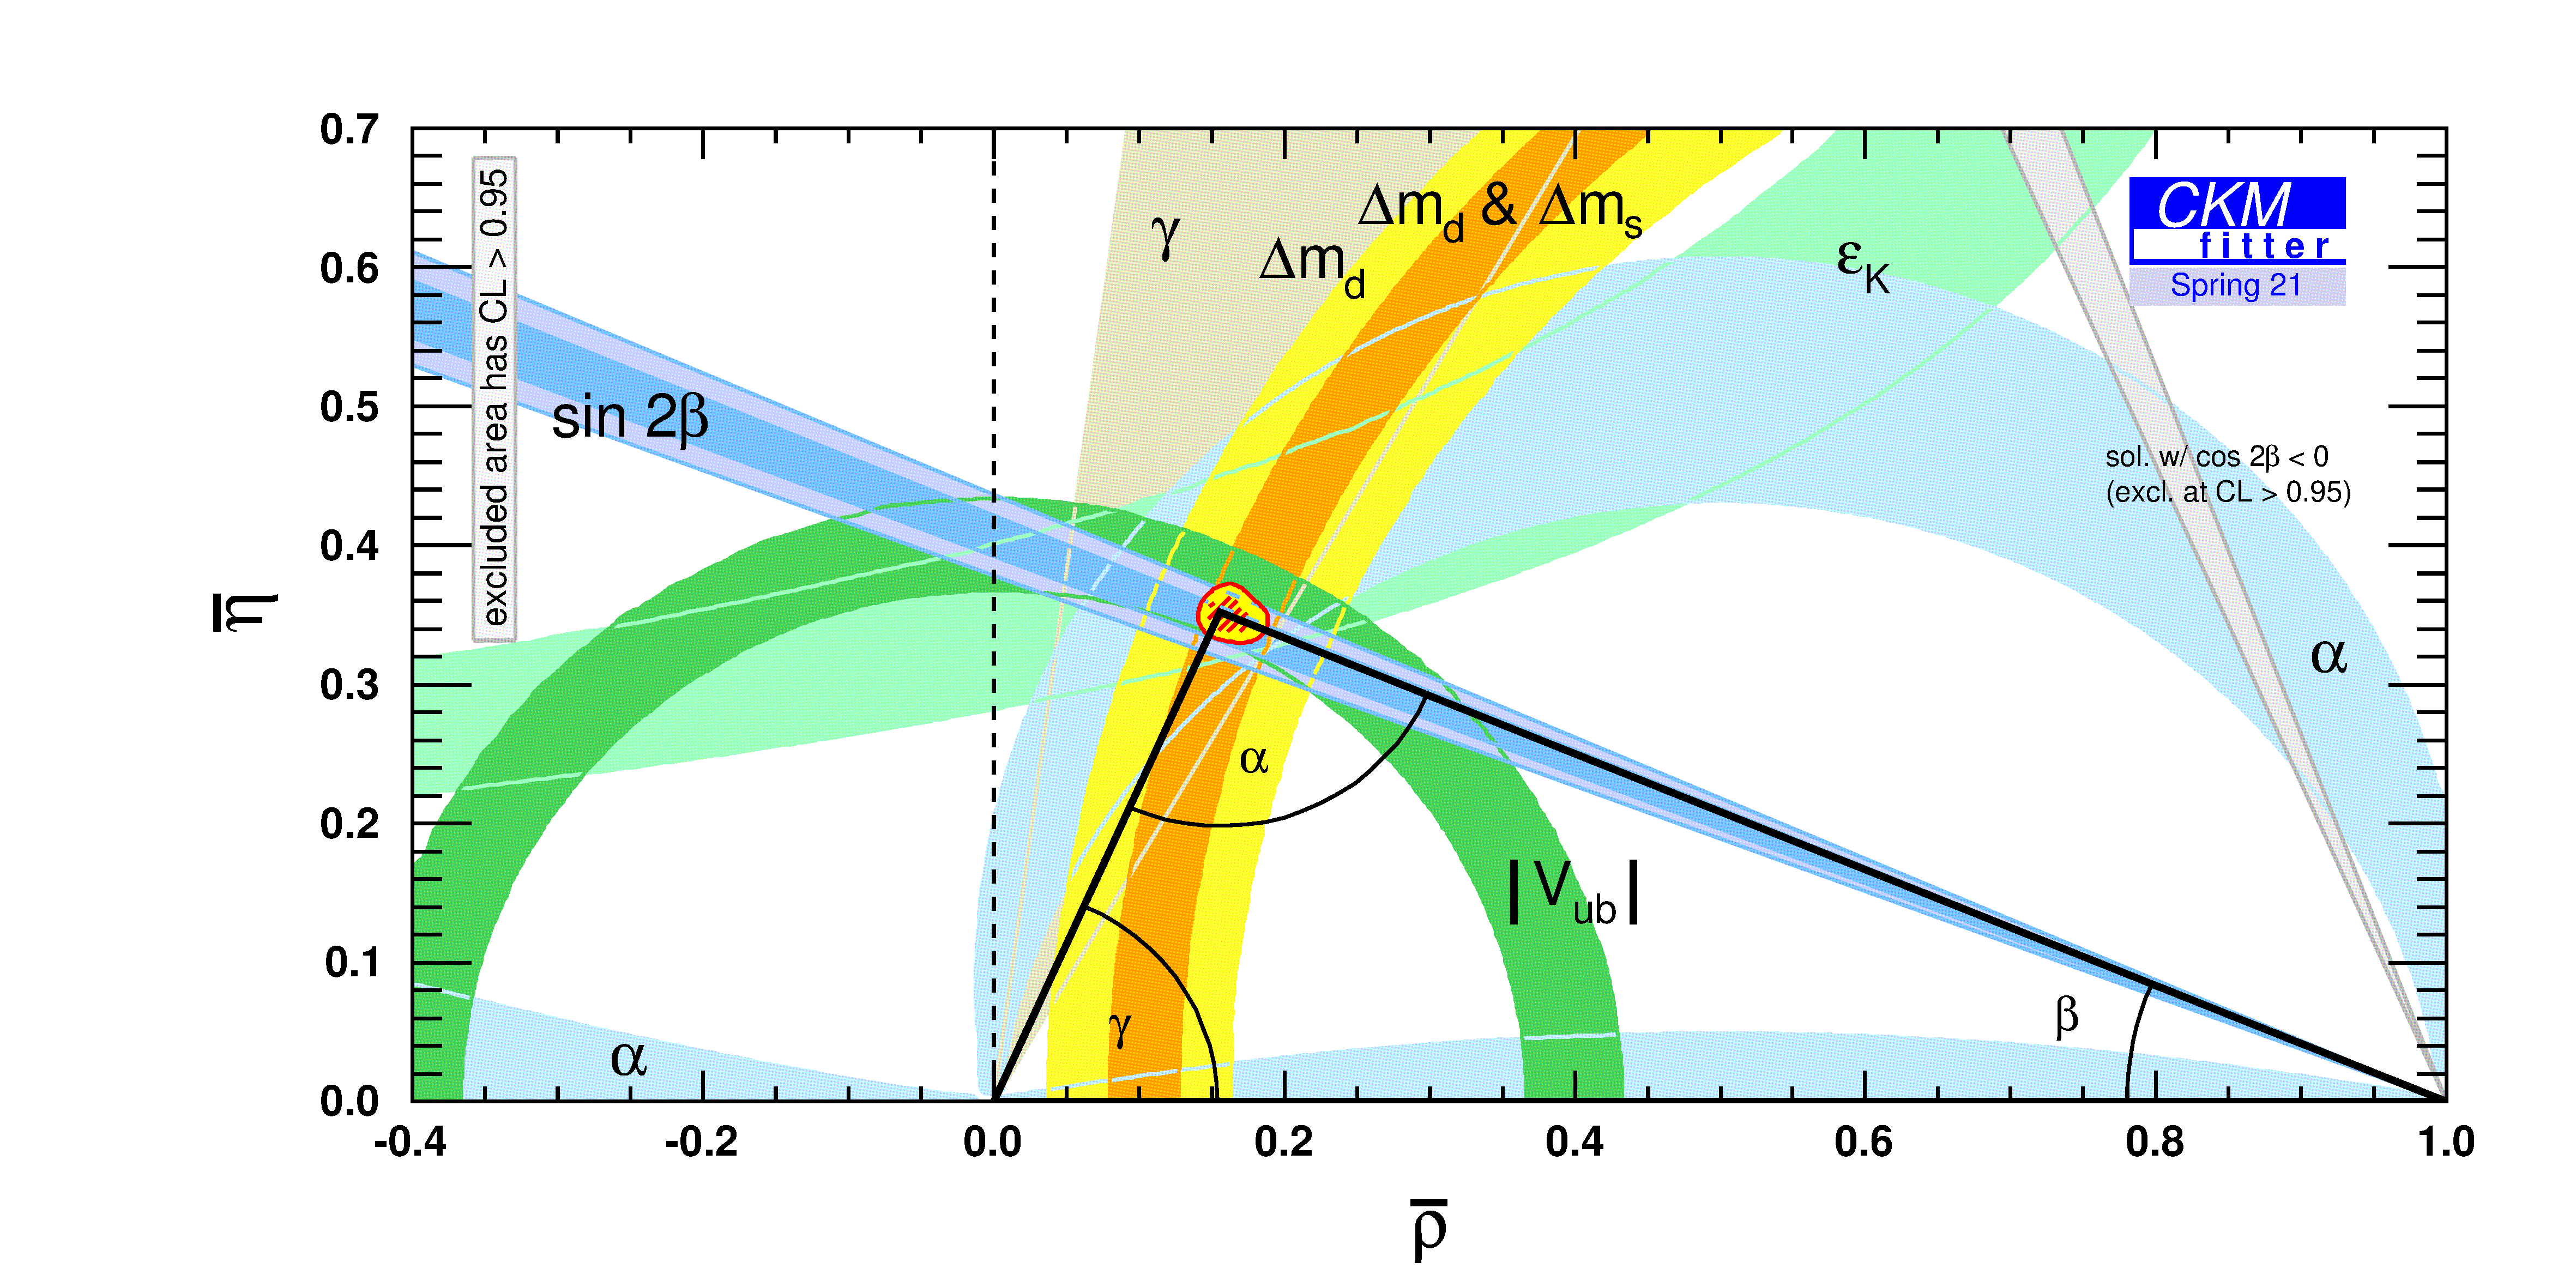
\includegraphics[width = 0.70\textwidth]{Plots/ckmfitter2.pdf}
  \end{figure}
  \vspace{-0.5cm}
  \begin{center}
    \tiny{CKMfitter Group (J. Charles et al.), Eur. Phys. J. C41, 1-131 (2005)}
  \end{center}
\end{frame}

\begin{frame}{Introduction and motivation}
  \vspace{0.5cm}
  \begin{itemize}
    \setlength\itemsep{1.2em}
    \item{$B^\pm\to[K^+K^-\pi^+\pi^-]_D K^\pm$ was first proposed by J. Rademacker and G. Wilkinson}
    \begin{itemize}
      \item{\href{https://arxiv.org/abs/hep-ph/0611272}{Phys. Lett. B647 (2007) 400}}
      \item{Expected $\gamma$ precision from FOCUS amplitude model with $1000$ $B^\pm\to DK^\pm$ candidates: $14^\circ$}
    \end{itemize}
    \item{Recent state of the art amplitude analysis by LHCb:}
    \begin{itemize}
      \item{\href{https://arxiv.org/abs/1811.08304}{JHEP 02 (2019) 126}}
      \item{Develop a suitable binning scheme}
    \end{itemize}
    \item{Anticipate $20$ fb$^{-1}$ of $\psi(3770)$ data from BESIII by end of 2023}
    \begin{itemize}
      \item{Allows for a direct strong phase measurements of $D^0\to K^+K^-\pi^+\pi^-$}
      \item{Final $\gamma$ measurement will be model independent}
    \end{itemize}
  \end{itemize}
\end{frame}

\section{Theory of BPGGSZ method}

\begin{frame}{Theory of BPGGSZ method}
  \begin{itemize}
    \item{$B^\pm\to Dh^\pm$ amplitude:}
  \end{itemize}
  \begin{center}
    $\mathcal{A}(B^-) = \mathcal{A}(D^0) + r_Be^{i(\delta_B - \gamma)}\mathcal{A}(\bar{D^0})$ \\
    $\mathcal{A}(B^+) = \mathcal{A}(\bar{D^0}) + r_Be^{i(\delta_B + \gamma)}\mathcal{A}(D^0)$ \\
  \end{center}
  \begin{itemize}
    \item{$\mathcal{A}(D^0)$ and $\mathcal{A}(\bar{D^0})$ depend on $D$ phase space}
    \item{Strong-phase difference of $D^0$ and $\bar{D^0}$ decays inaccessible at LHCb}
    \item{Model-independent measurement: Integrate over bins of phase space}
  \end{itemize}
  \begin{block}{Event yield in bin $i$}
    $N^-_i = h_{B^-}\Big(F_i + \big(x_-^2 + y_-^2\big)\bar{F_i} + 2\sqrt{F_i\bar{F_i}}\big(x_-c_i + y_-s_i\big)\Big)$
    $N^+_{-i} = h_{B^+}\Big(F_i + \big(x_+^2 + y_+^2\big)\bar{F_i} + 2\sqrt{F_i\bar{F_i}}\big(x_+c_i + y_+s_i\big)\Big)$
  \end{block}
\end{frame}

\begin{frame}{Theory of BPGGSZ method}
  \begin{block}{Event yield in bin $i$}
    \scriptsize
    $N^-_i = h_{B^-}\big(F_i + (x_-^2 + y_-^2)\bar{F_i} + 2\sqrt{F_i\bar{F_i}}(x_-c_i + y_-s_i)\big)$ \\
    $N^+_{-i} = h_{B^+}\big(F_i + (x_+^2 + y_+^2)\bar{F_i} + 2\sqrt{F_i\bar{F_i}}(x_+c_i + y_+s_i)\big)$
  \end{block}
  \begin{itemize}
    \item{CP observables:}
    \begin{itemize}
      \item{$x_\pm^{DK} = r_B^{DK}\cos(\delta_B^{DK}\pm\gamma)$, \quad $y_\pm^{DK} = r_B^{DK}\sin(\delta_B^{DK}\pm\gamma)$}
      \item{$x_\xi^{D\pi} = \Re(\xi^{D\pi})$, $y_\xi^{D\pi} = \Im(\xi^{D\pi})$ $\quad\quad\Big(\xi^{D\pi} = \frac{r_B^{D\pi}}{r_B^{DK}}e^{i(\delta_B^{D\pi} - \delta_B^{DK})}\Big)$}
    \end{itemize}
    \item{Fractional bin yield:}
    \begin{itemize}
      \item{$F_i = \frac{\int_i\dd{\Phi}|\mathcal{A}(D^0)|^2}{\sum_j\int_j\dd{\Phi}\abs{\mathcal{A}(D^0)}^2}$}
      \item{Floated in the fit, mostly constrained by $B^\pm\to D\pi^\pm$}
    \end{itemize}
  \end{itemize}
  \begin{itemize}
    \item{Amplitude averaged strong phases:}
    \begin{center}
      $c_i = \frac{\int_i\dd{\Phi}|\mathcal{A}(D^0)||\mathcal{A}(\bar{D^0})|\cos(\delta_D)}{\sqrt{\int_i\dd{\Phi}\abs{\mathcal{A}(D^0)}^2\int_i\dd{\Phi}\abs{\mathcal{A}(\bar{D^0})}^2}}$ \quad $s_i = \frac{\int_i\dd{\Phi}|\mathcal{A}(D^0)||\mathcal{A}(\bar{D^0})|\sin(\delta_D)}{\sqrt{\int_i\dd{\Phi}\abs{\mathcal{A}(D^0)}^2\int_i\dd{\Phi}\abs{\mathcal{A}(\bar{D^0})}^2}}$
    \end{center}
  \end{itemize}
\end{frame}

\section{Binning scheme}

\begin{frame}{Binning scheme}
  \vspace{0.0cm}
  {\Large A binning scheme must satisfy the following:}
  \begin{itemize}
    \item{Minimal dilution of strong phases when integrating over bins}
    \item{Enhance interference between $B^\pm\to D^0h^\pm$ and $B^\pm\to\bar{D^0}h^\pm$}
  \end{itemize}
  \vspace{0.4cm}
  {\Large How to bin a 5-dimensional phase space?}
  \begin{itemize}
    \item{Generate C++ code for LHCb amplitude model using AmpGen\footnote{\href{https://github.com/GooFit/AmpGen}{AmpGen} by Tim Evans}}
    \item{For each $B^\pm$ candidate, calculate}
  \end{itemize}
  \begin{center}
    {\Large $\frac{\mathcal{A}(D^0)}{\mathcal{A}(\bar{D^0})} = r_De^{i\delta_D}$}
  \end{center}
  \begin{itemize}
    \item{Bin along $\delta_D$ and $r_D$, maximize $Q$-value to optimize}
  \end{itemize}
\end{frame}

\begin{frame}{Binning scheme}
  \begin{figure}
    \centering
    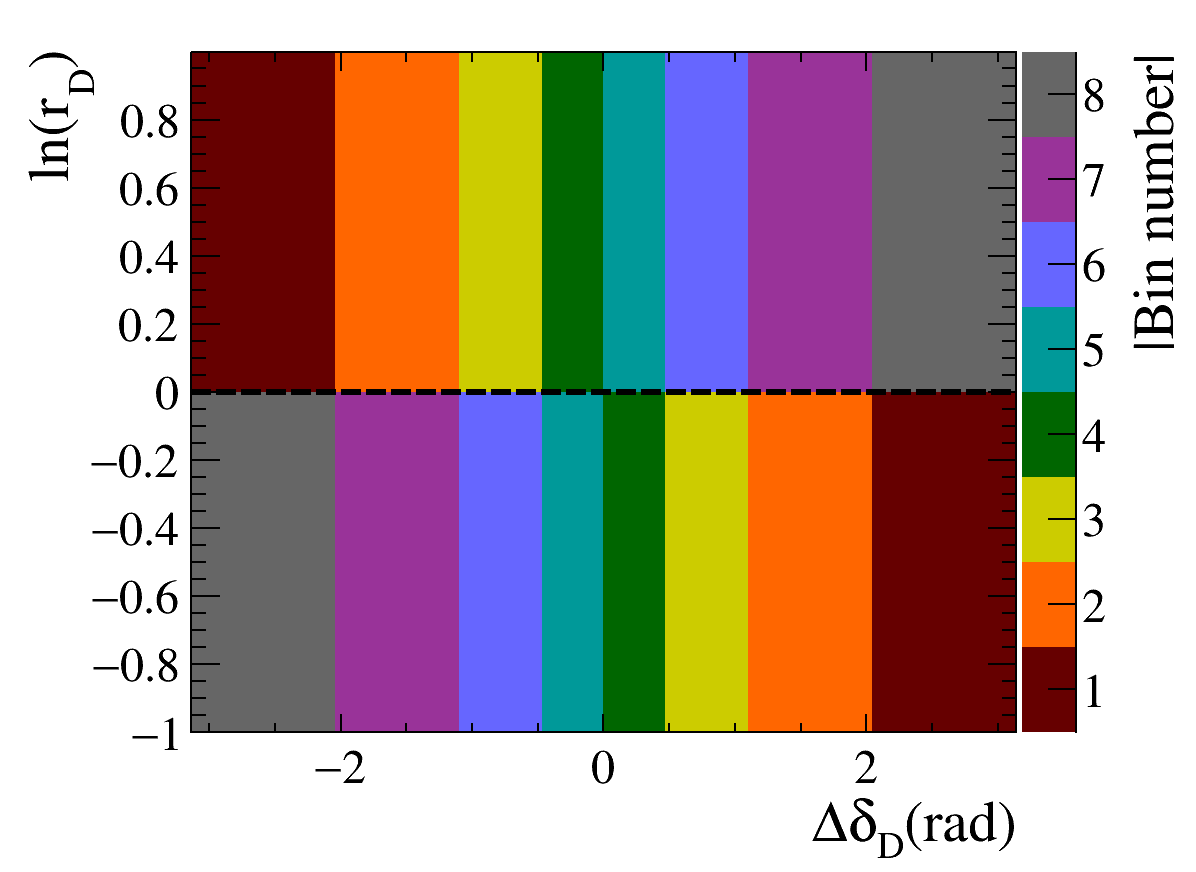
\includegraphics[width = 0.7\textwidth]{Plots/BinningSchemePlot_8Bins.png}
  \end{figure}
  \vspace{-1.0cm}
  \begin{center}
    $Q = 0.90$ \\
    Bins $i < 0$ on top, $i > 0$ below
  \end{center}
\end{frame}

\section{Quasi-GLW method}

\begin{frame}{The quasi-GLW method}
  \begin{itemize}
    \setlength\itemsep{0.5em}
    \item{Statistically independent analysis without phase space binning}
    \begin{itemize}
      \item{BPGGSZ looks at relative bin yields}
      \item{Quasi-GLW observables depend on absolute yields}
    \end{itemize}
    \item{Charge asymmetry:}
    \begin{center}
      $A_h = \frac{\Gamma(B^-\to D h^-) - \Gamma(B^+\to D h^+)}{\Gamma(B^-\to D h^-) + \Gamma(B^+\to D h^+)}$
    \end{center}
    \item{$B\to DK$ vs $B\to D\pi$ double ratio:}
    \begin{center}
      $R_{\rm CP} = \frac{R_{hh\pi\pi}}{R_{K\pi\pi\pi}}, \quad R = \frac{\Gamma(B^-\to D K^-) + \Gamma(B^+\to D K^+)}{\Gamma(B^-\to D\pi^-) + \Gamma(B^+\to D\pi^+)}$
    \end{center}
  \end{itemize}
  \begin{block}{CP observables and physics parameters}
    $A_h = \frac{2r_B^{Dh}(2F_+ - 1)\sin(\delta_B^{Dh})\sin(\gamma)}{1 + (r_B^{Dh})^2 + 2r_B^{Dh}(2F_+ - 1)\cos(\delta_B^{Dh})\cos(\gamma)}$, \\~\\
    $R_{\rm CP} = 1 + (r_B^{Dh})^2 + 2r_B^{Dh}(2F_+ - 1)\cos(\delta_B^{Dh})\cos(\gamma)$
  \end{block}
\end{frame}

\section{Selection}

\begin{frame}{Selection}
  \begin{enumerate}
    \setlength\itemsep{1.0em}
    \item{Initial cuts: Trigger requirements, mass cuts, bachelor $p$, etc}
    \begin{itemize}
      \item{$D$ mass window: $25$ MeV}
      \item{$B^\pm$ mass fit range: $[5080, 5700]$ MeV}
    \end{itemize}
    \item{BDT: Efficient combinatorial background rejection}
    \item{Final cuts: PID cuts, flight significance cuts, $K_S$ veto, etc}
    \begin{itemize}
      \item{PIDK cut at 4 to separate $B^\pm\to DK^\pm$ and $B^\pm\to D\pi^\pm$}
      \item{Flight significance at $2$ to reduce charmless backgrounds}
      \item{Pick BDT cut that minimised statistical sensitity of $\gamma$}
    \end{itemize}
  \end{enumerate}
  \vspace{0.5cm}
  \begin{figure}
    \centering
    \vspace{-0.2cm}
    \begin{subfigure}{0.5\textwidth}
      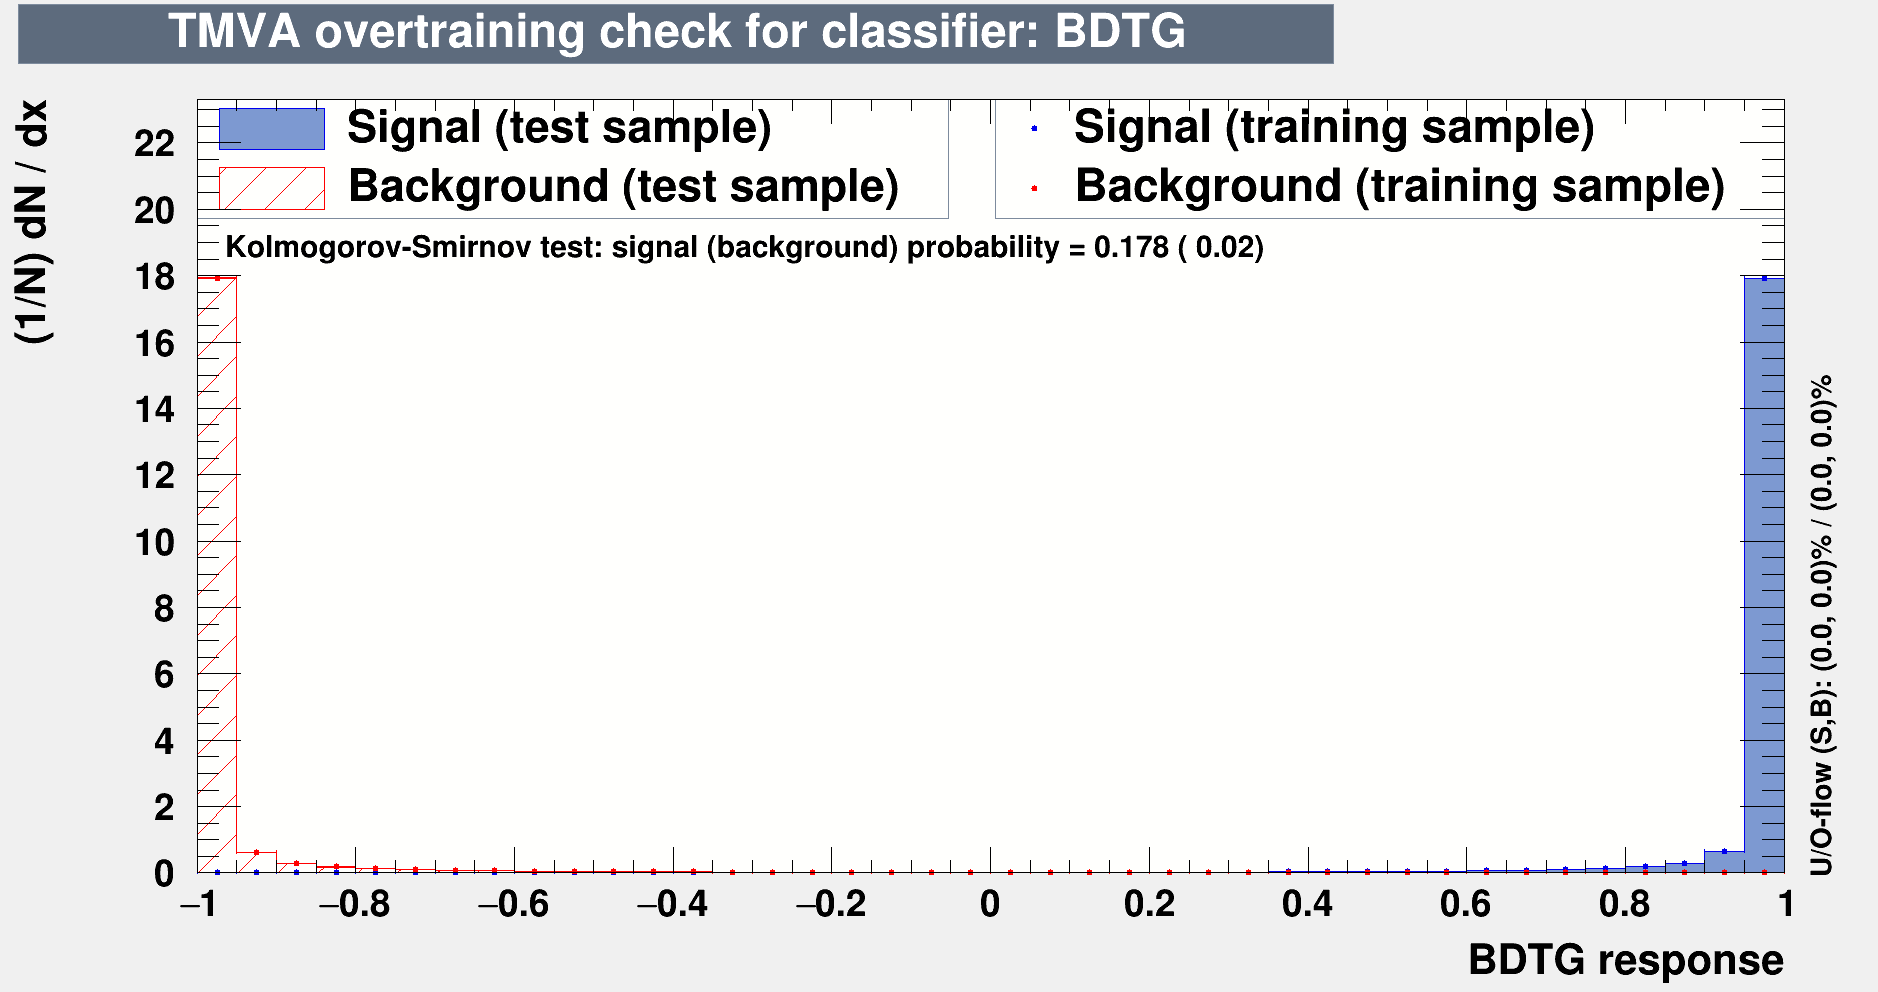
\includegraphics[width = 1.0\textwidth]{Plots/overtrain_BDTG.png}
      \caption{BDT output}
    \end{subfigure}%
    \begin{subfigure}{0.5\textwidth}
      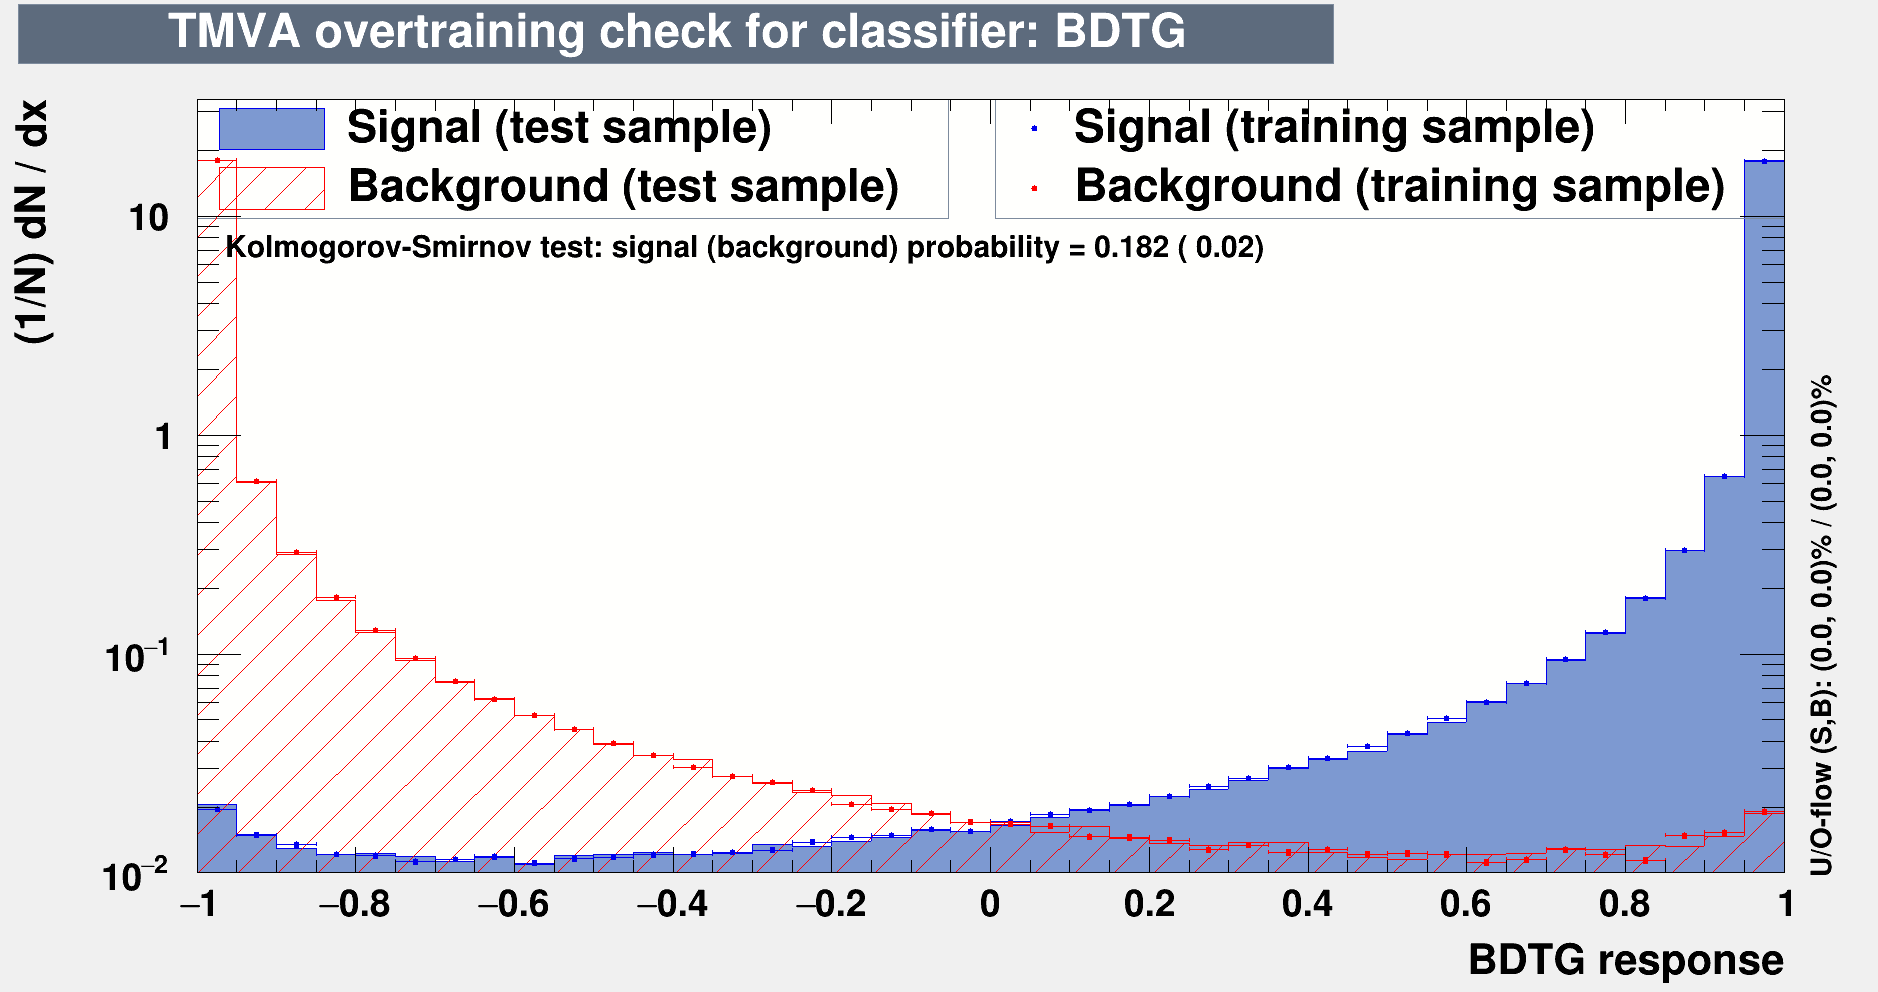
\includegraphics[width = 1.0\textwidth]{Plots/overtrain_BDTG_log.png}
      \caption{BDT output on a logarithmic scale}
    \end{subfigure}
  \end{figure}
\end{frame}

\section{Backgrounds}

\begin{frame}{Summary of backgrounds}
  \begin{itemize}
    \item{Partially reconstructed $B$ decays}
    \begin{itemize}
      \item{Modelled in the fit with HILL/HORNSdini shapes}
    \end{itemize}
    \item{Combinatorial}
    \begin{itemize}
      \item{Floating exponential}
    \end{itemize}
    \item{CF $D^0\to K^-\pi^+\pi^-\pi^+$ and semi-leptonic $D^0\to K^-(X)l^+\nu_l$ background}
    \begin{itemize}
      \item{Small, assign systematic}
    \end{itemize}
    \item{Charmless}
    \begin{itemize}
      \item{Fix from sideband}
    \end{itemize}
    \item{CF $D^0\to K^-\pi^+\pi^-\pi^+\pi^0$ background}
    \begin{itemize}
      \item{Not negligible!}
    \end{itemize}
  \end{itemize}
\end{frame}

\begin{frame}{$D^0\to K^-\pi^+\pi^-\pi^+\pi^0$ partially reconstructed mis-ID}
  \begin{itemize}
    \setlength\itemsep{0.0em}
    \item{Missing $\pi^0$ and $\pi\to K$ mis-ID}
    \item{Float yield relative to $B\to D^*h$ background}
  \end{itemize}
  \begin{figure}
    \centering
    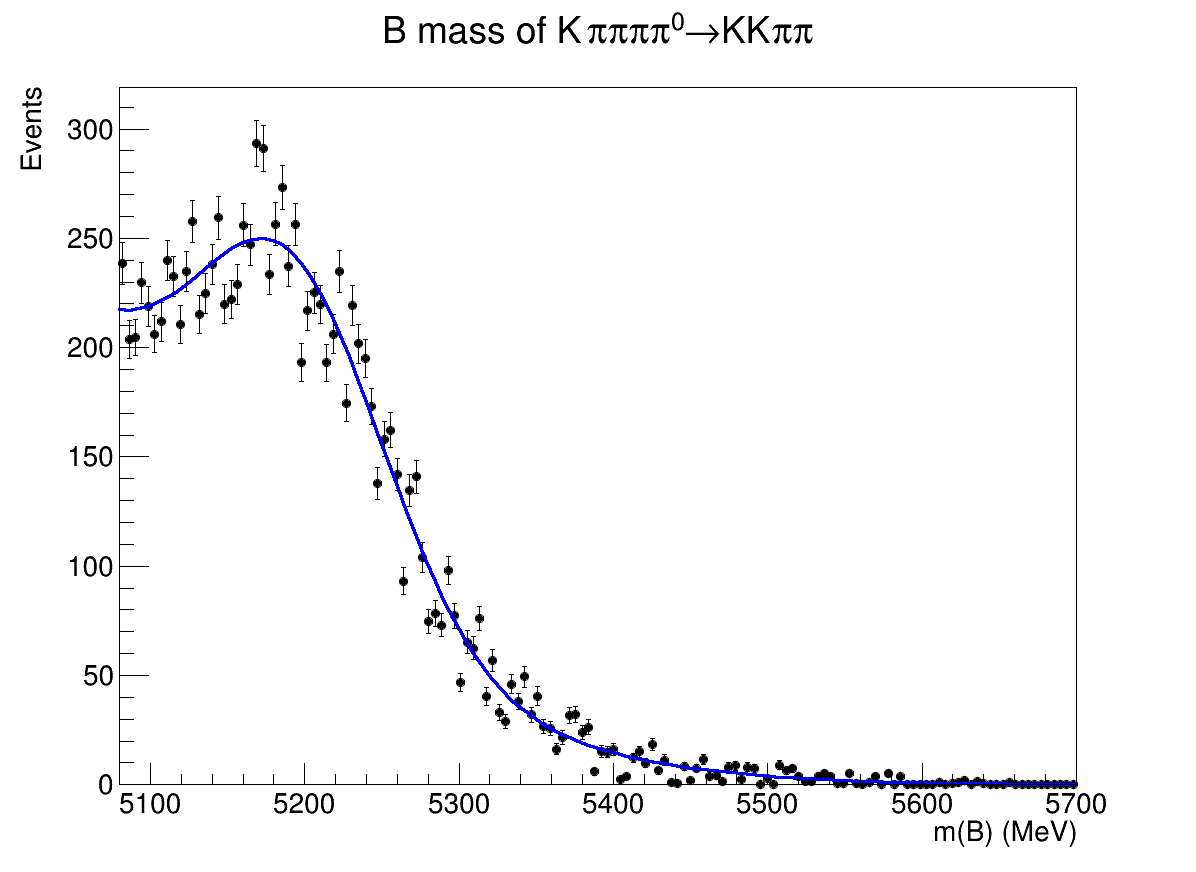
\includegraphics[width = 0.8\textwidth]{Plots/Kpipipipi0BMassB2DpiD2Kpipipi.png}
  \end{figure}
\end{frame}

\section{Global fit}

\begin{frame}{Global fit}
  \begin{figure}
    \centering
    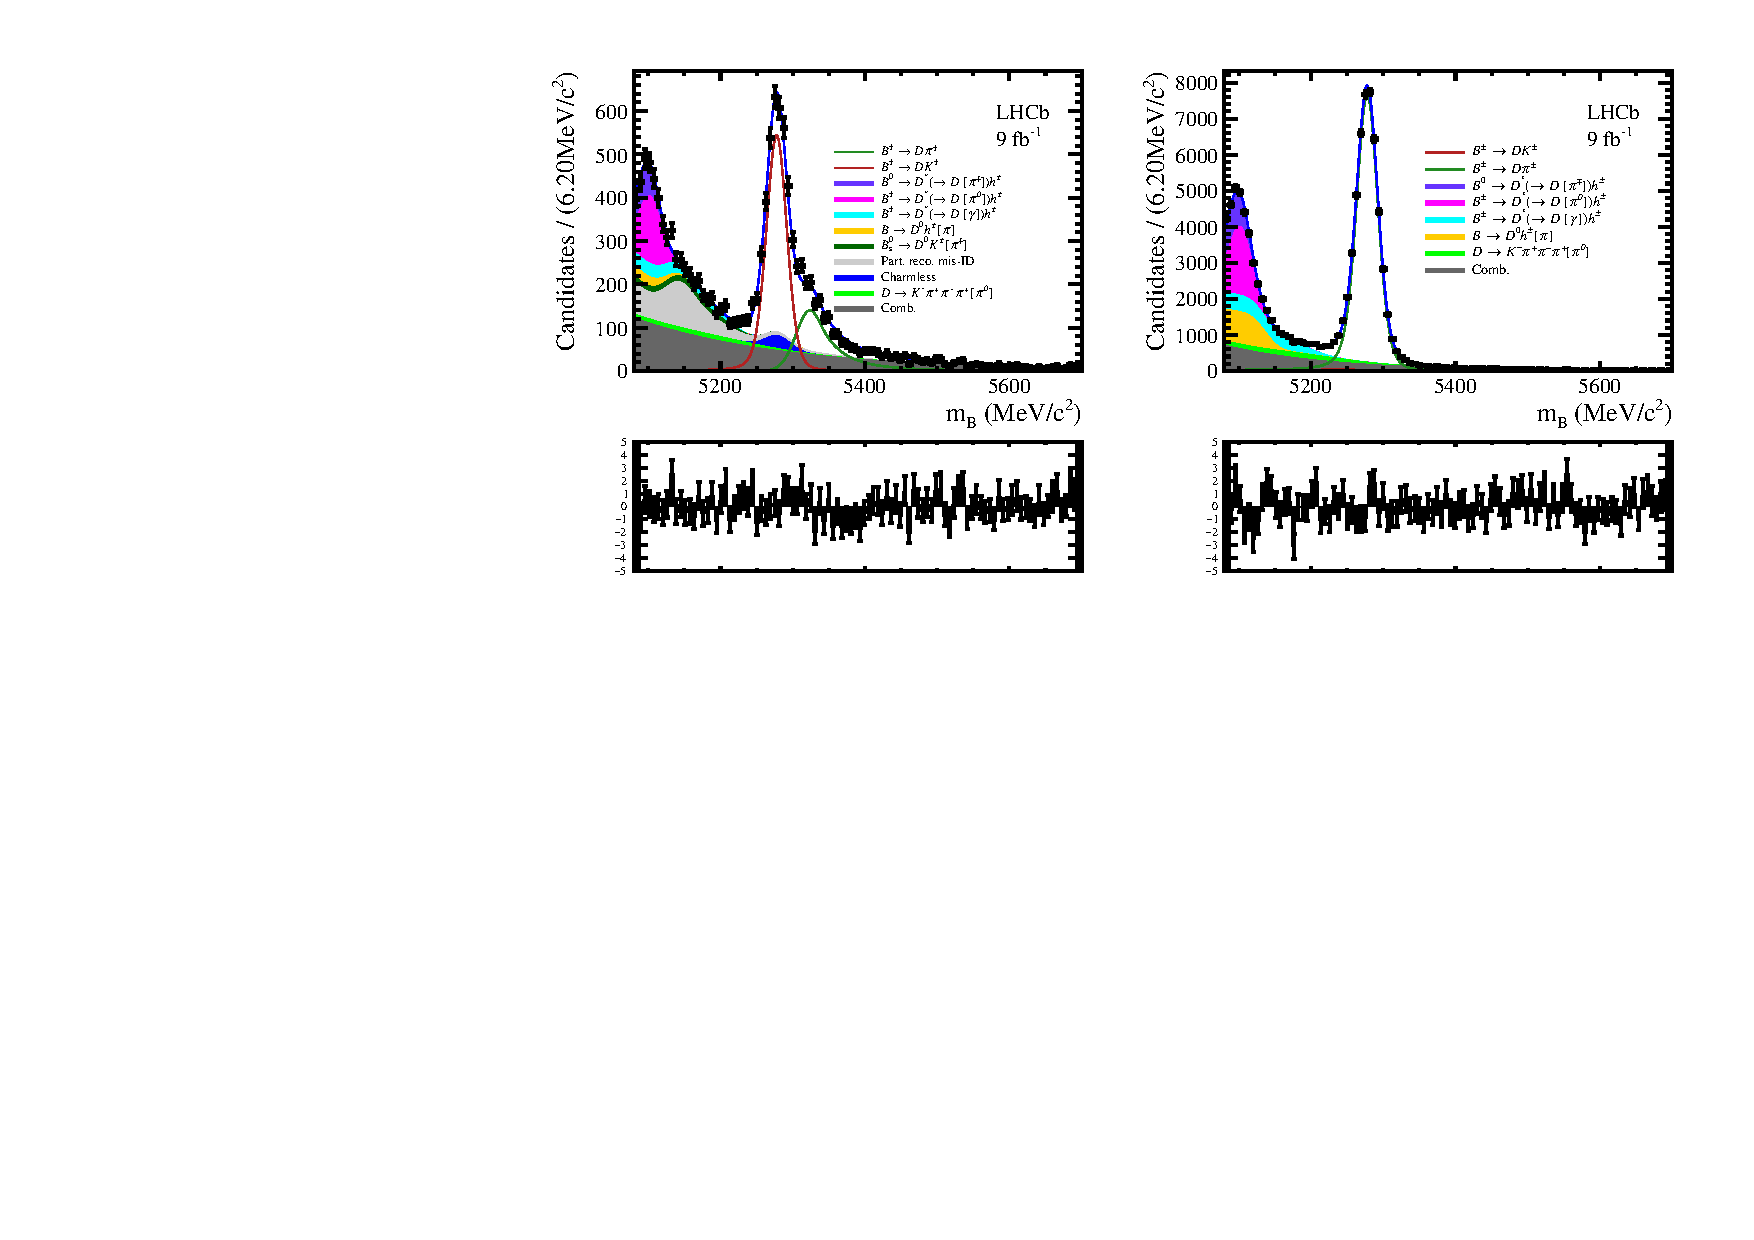
\includegraphics[width = 1.0\textwidth]{Plots/d2kkpipi_fiveL_allDP.pdf}
    \caption{$B^\pm\to DK^\pm$ channel (left) and $B^\pm\to D\pi^\pm$ channel (right)}
  \end{figure}
  \vspace{-0.5cm}
  \begin{itemize}
    \item{$B^\pm\to DK^\pm$ yield: $\SI{3026(38)}{}$}
    \item{$B^\pm\to D\pi^\pm$ yield: $\SI{44349(218)}{}$}
  \end{itemize}
\end{frame}

\section{Quasi-GLW fit}

\begin{frame}{Fit split by charge}
  \begin{figure}
    \centering
    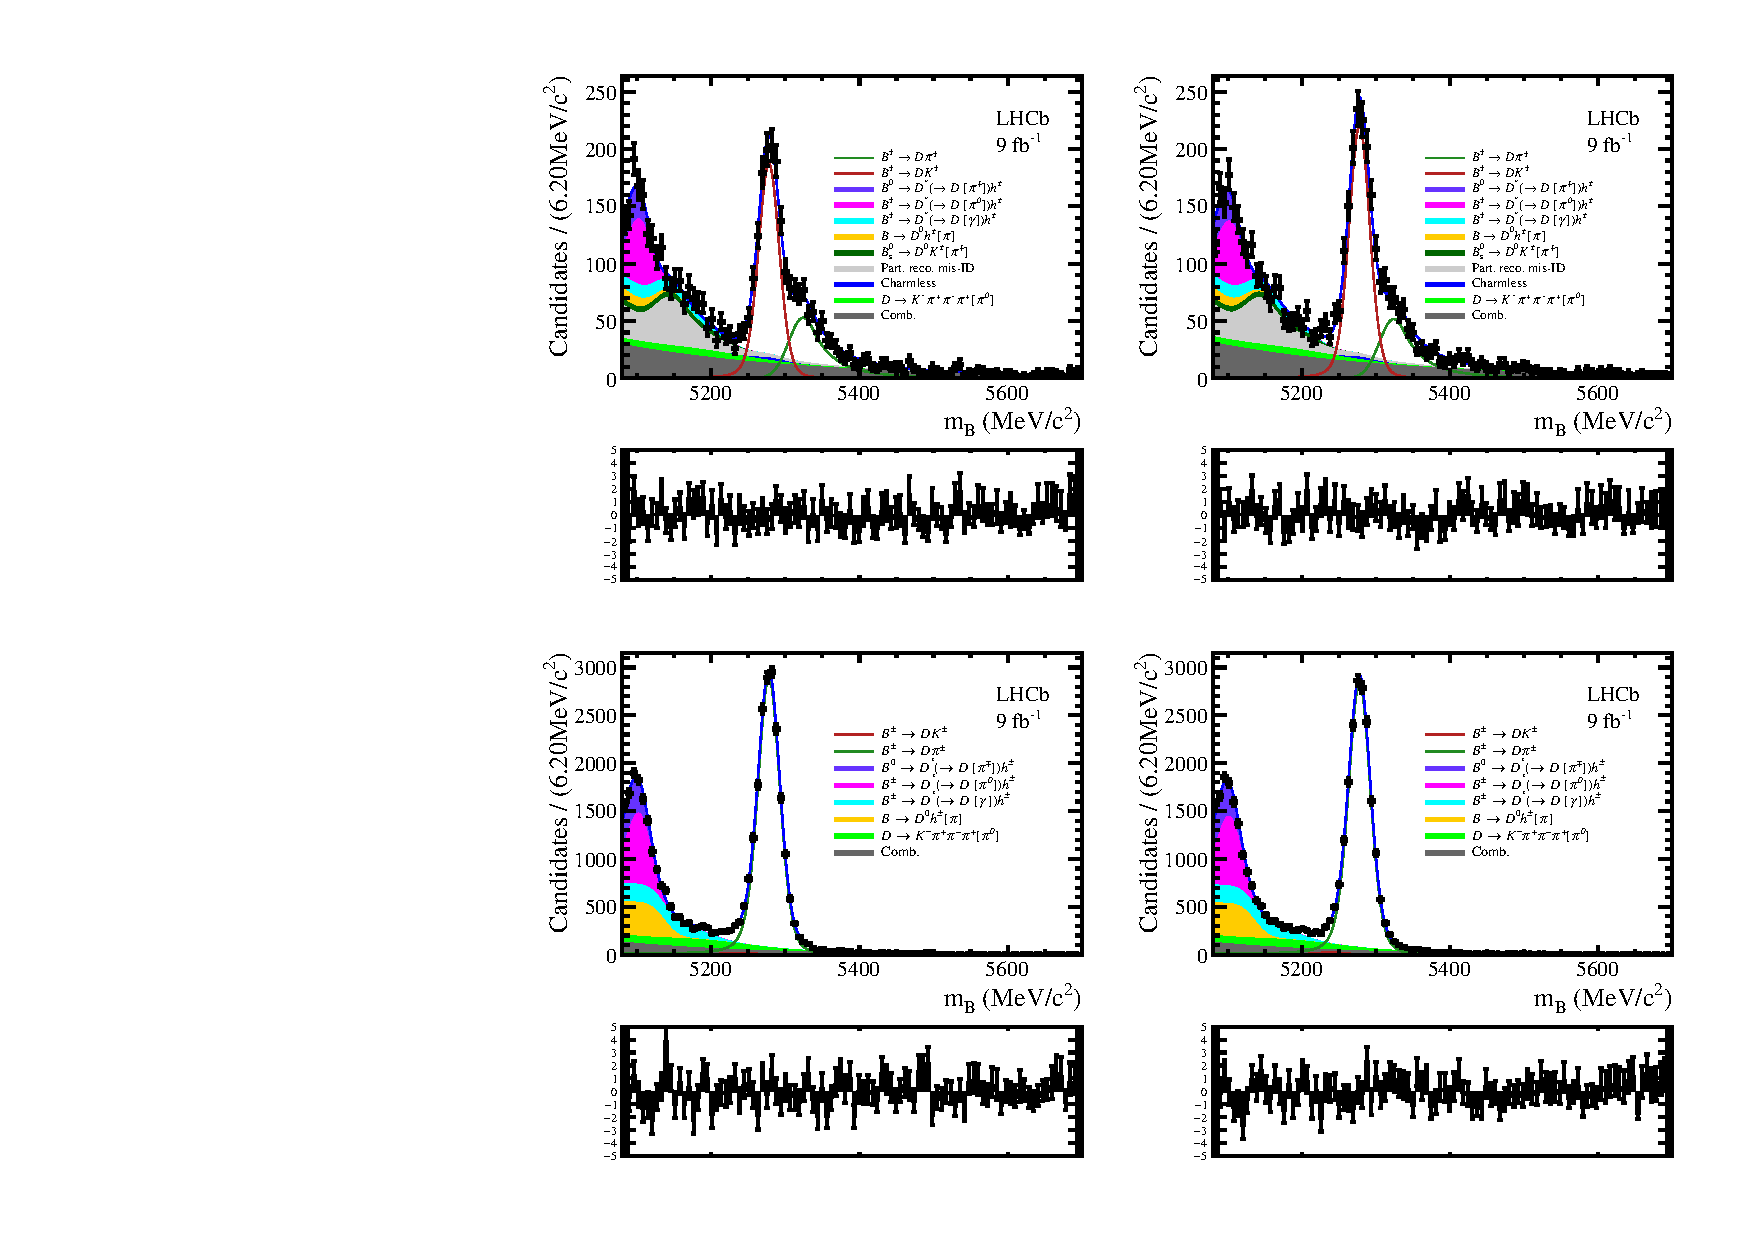
\includegraphics[width = 0.9\textwidth, clip = true, trim = {0 12.9cm 0 0}]{Plots/d2kkpipi_fiveL_allDP_GLW.pdf}
    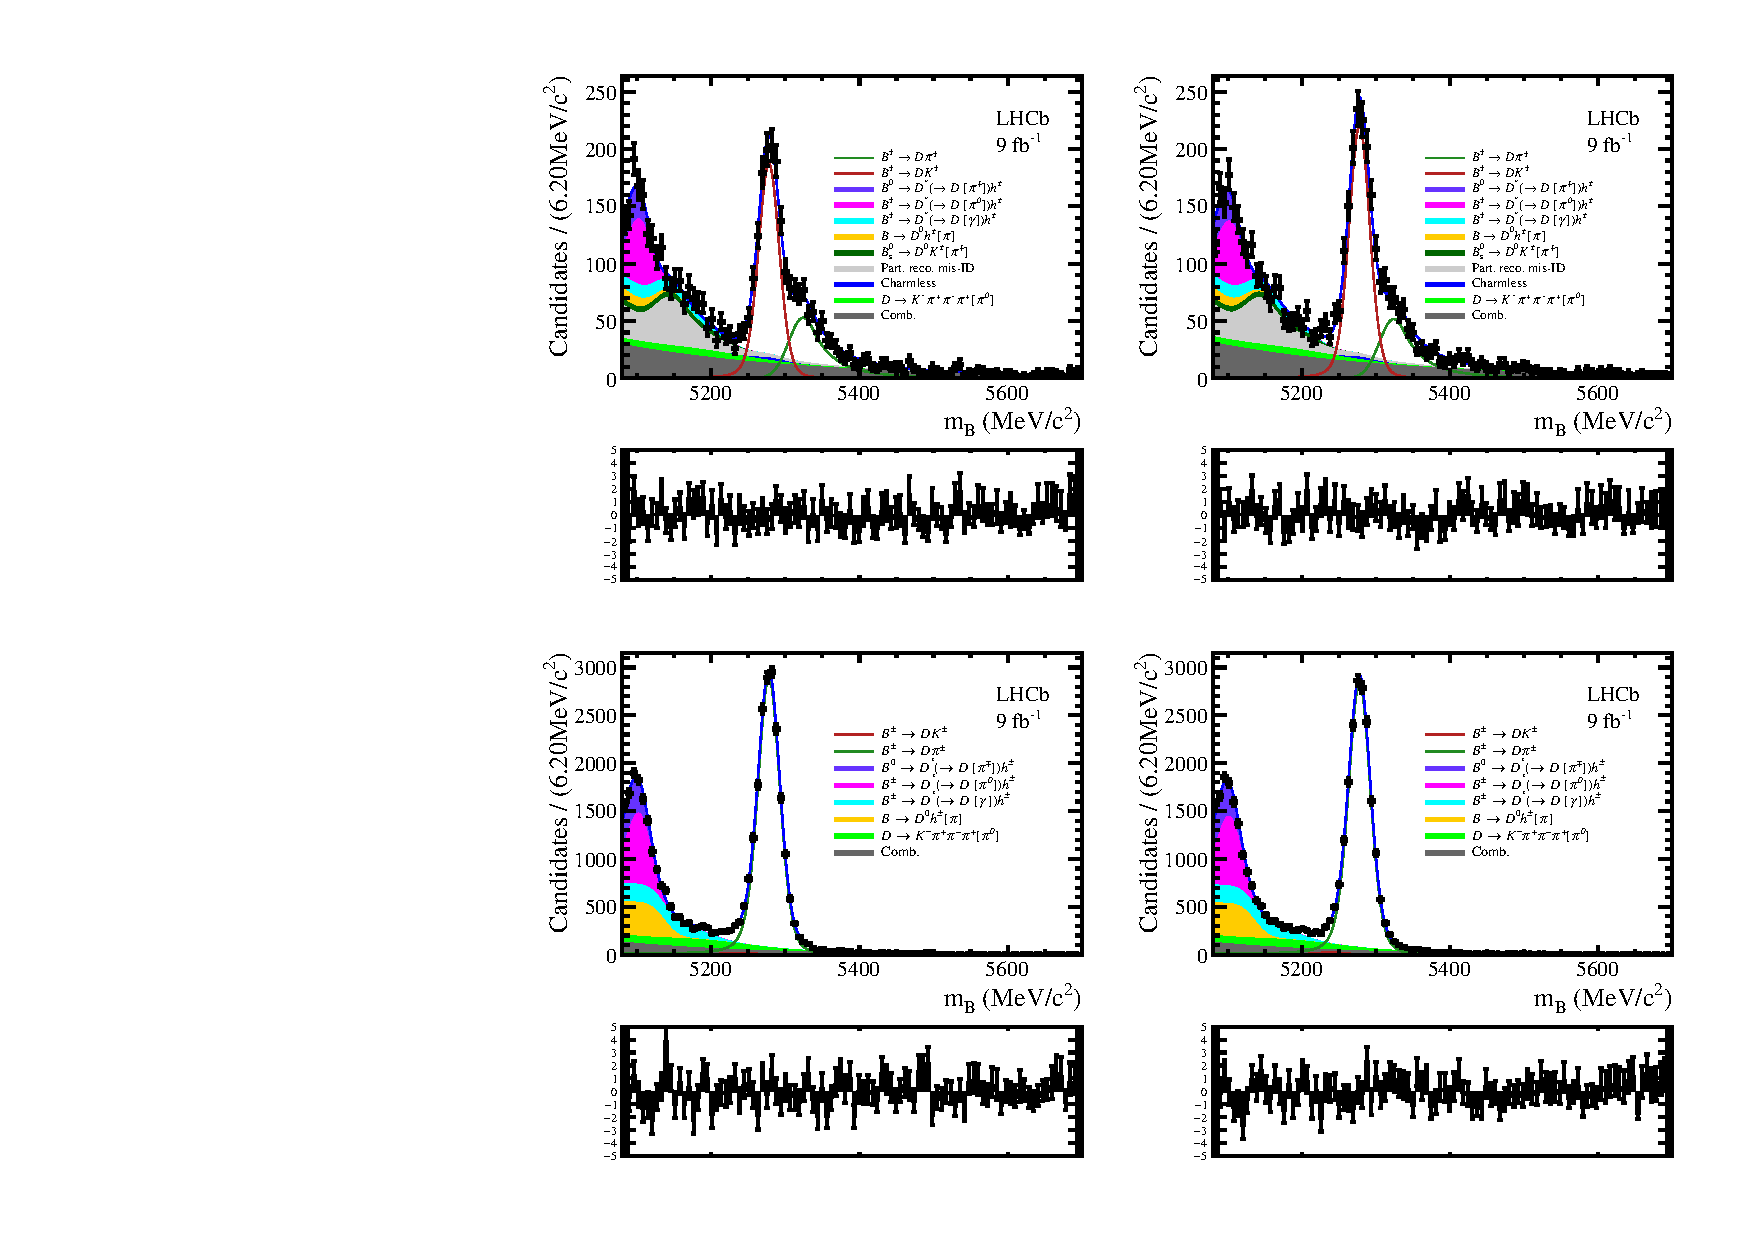
\includegraphics[width = 0.9\textwidth, clip = true, trim = {0 3cm 0 10cm}]{Plots/d2kkpipi_fiveL_allDP_GLW.pdf}
    \caption{$B^\pm\to (K^+K^-\pi^+\pi^-)Dh^\pm$}
  \end{figure}
\end{frame}

\begin{frame}{Fit split by charge}
  \begin{figure}
    \centering
    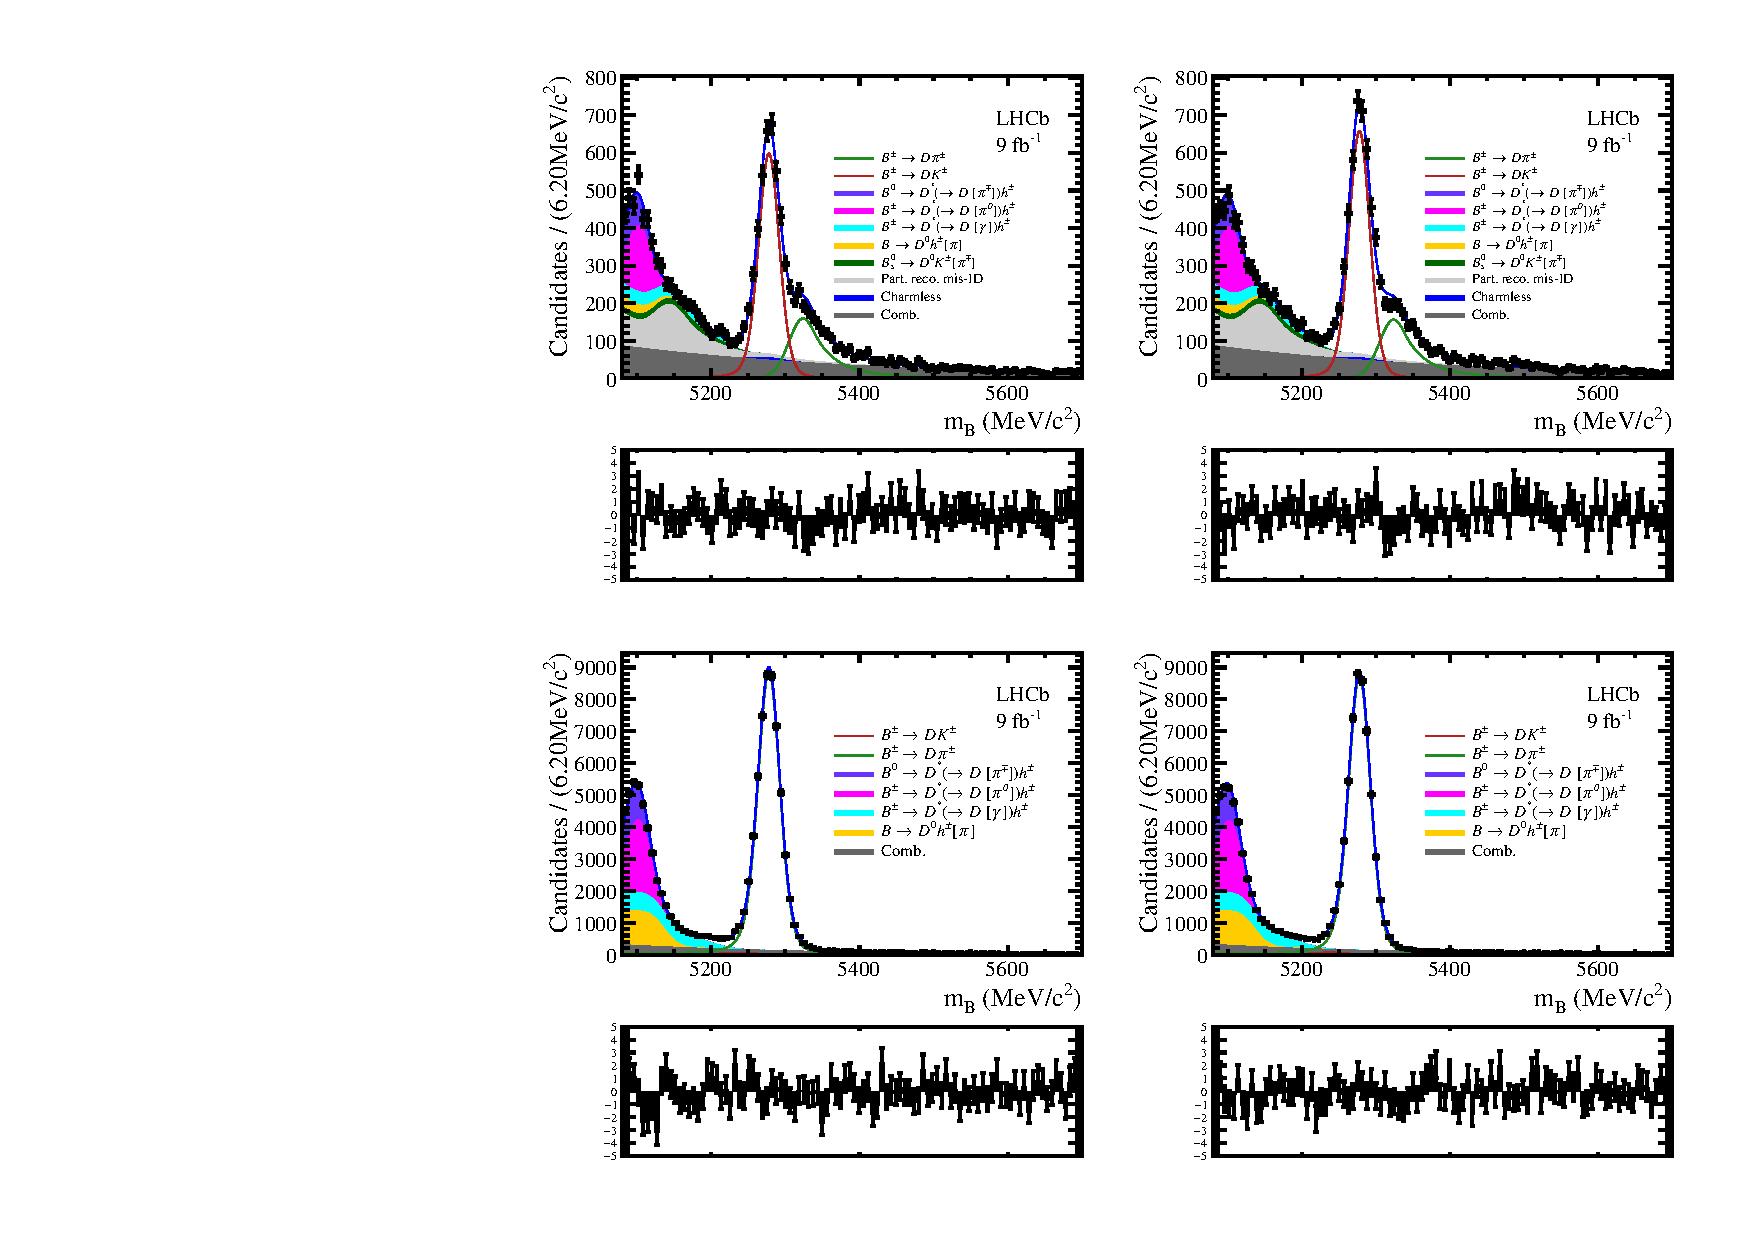
\includegraphics[width = 0.9\textwidth, clip = true, trim = {0 12.9cm 0 0}]{Plots/d2pipipipi_fiveL_allDP_GLW.pdf}
    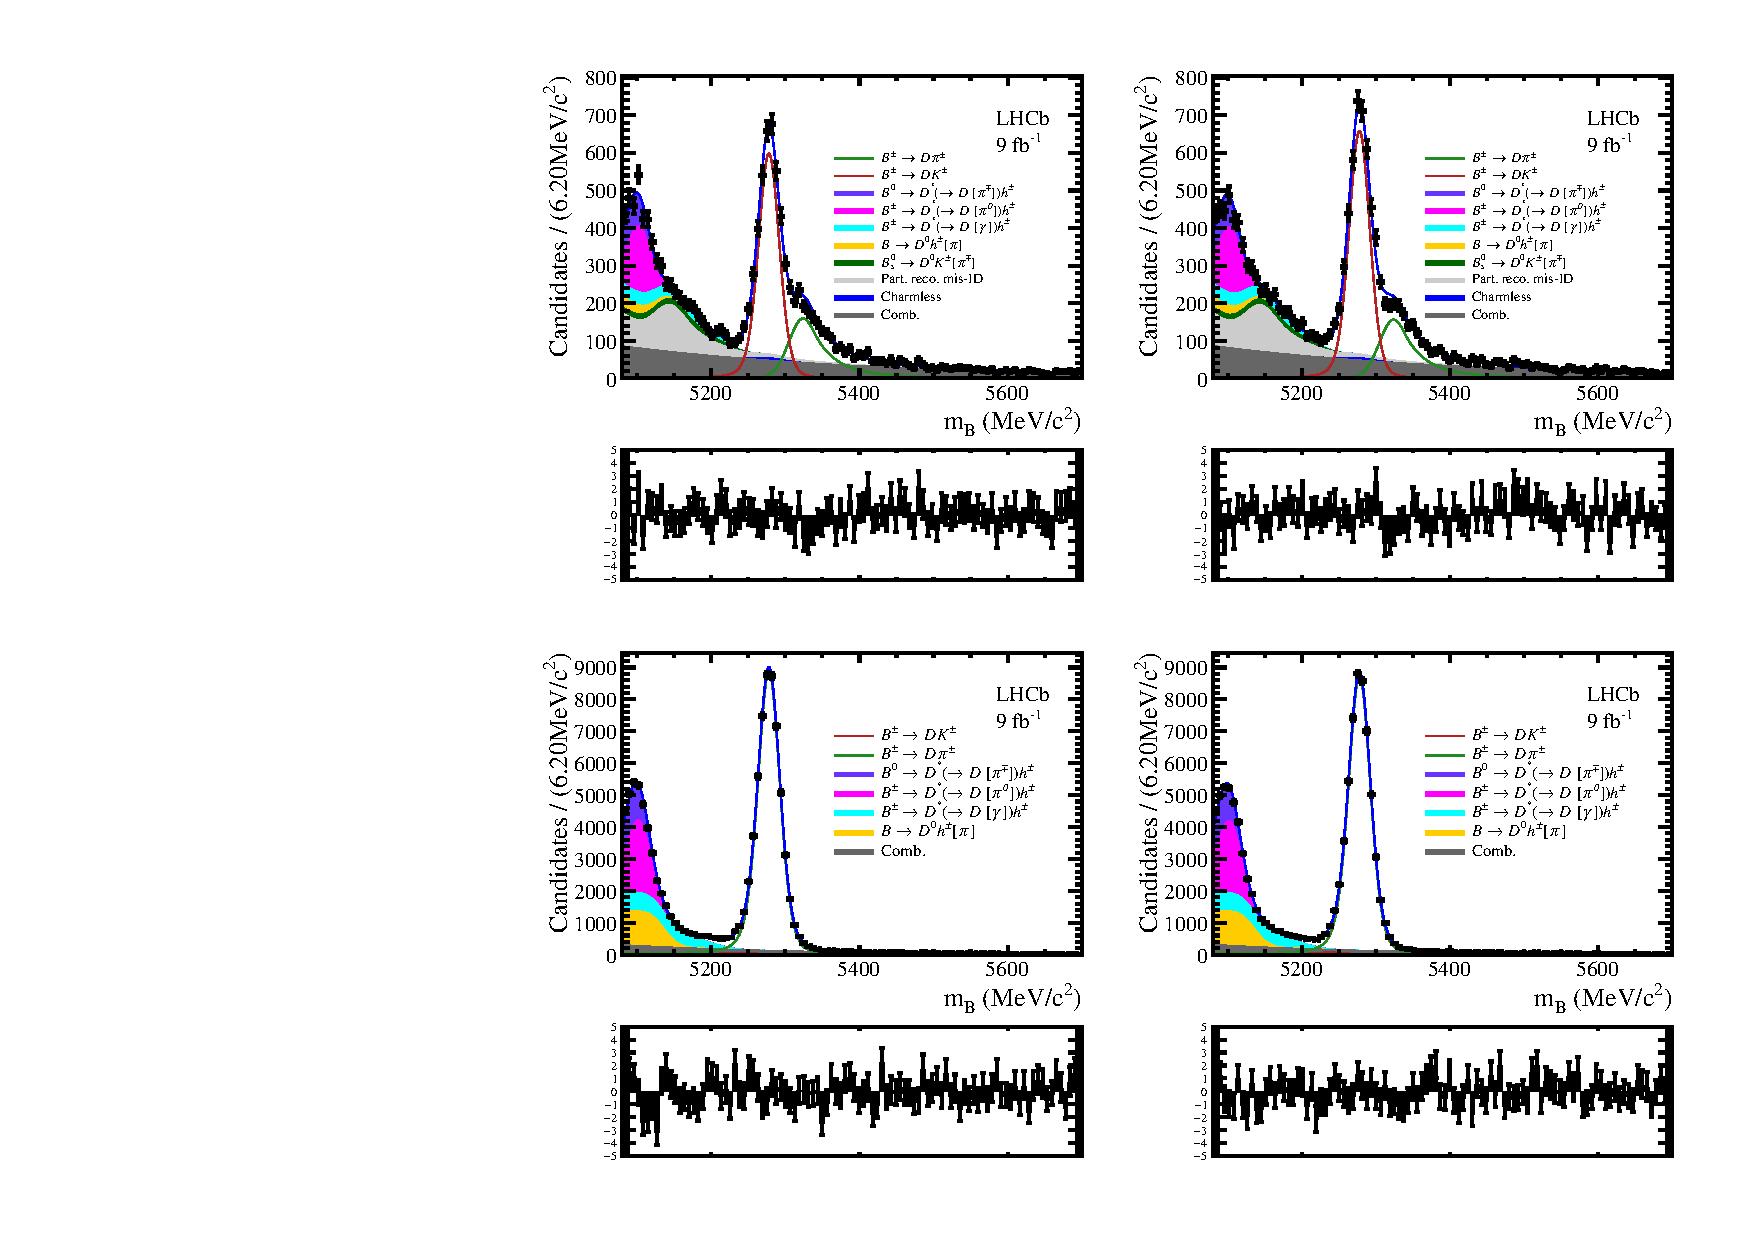
\includegraphics[width = 0.9\textwidth, clip = true, trim = {0 3cm 0 10cm}]{Plots/d2pipipipi_fiveL_allDP_GLW.pdf}
    \caption{$B^\pm\to (\pi^+\pi^-\pi^+\pi^-)Dh^\pm$}
  \end{figure}
\end{frame}

\section{CP fit}

\begin{frame}{CP fit setup}
  \begin{itemize}
    \item{Fix mass shape from global fit}
    \item{Split by $B^\pm$ charge and $D$ phase space bins}
    \begin{itemize}
      \item{Simultaneous fit with $64$ categories}
    \end{itemize}
    \item{Signal yields parameterised in terms of $x_\pm^{DK}$, $y_\pm^{DK}$ $x_\xi^{D\pi}$, $y_\xi^{D\pi}$ ($6$ parameters)}
    \item{Fractional bin yields $F_i$ are floating ($15$ parameter)}
    \item{Combinatorial background yield floated in each bin ($64$ parameters)}
    \item{Total partially reconstructed background yield floated in each bin ($64$ parameters)}
    \item{Normalisation of each charge and $B^\pm$ decay is floated ($4$ parameters)}
    \item{In total: $153$ free parameters}
  \end{itemize}
\end{frame}

\begin{frame}{CP fit results}
  \begin{figure}
    \centering
    \vspace{-0.2cm}
    \begin{subfigure}{0.5\textwidth}
      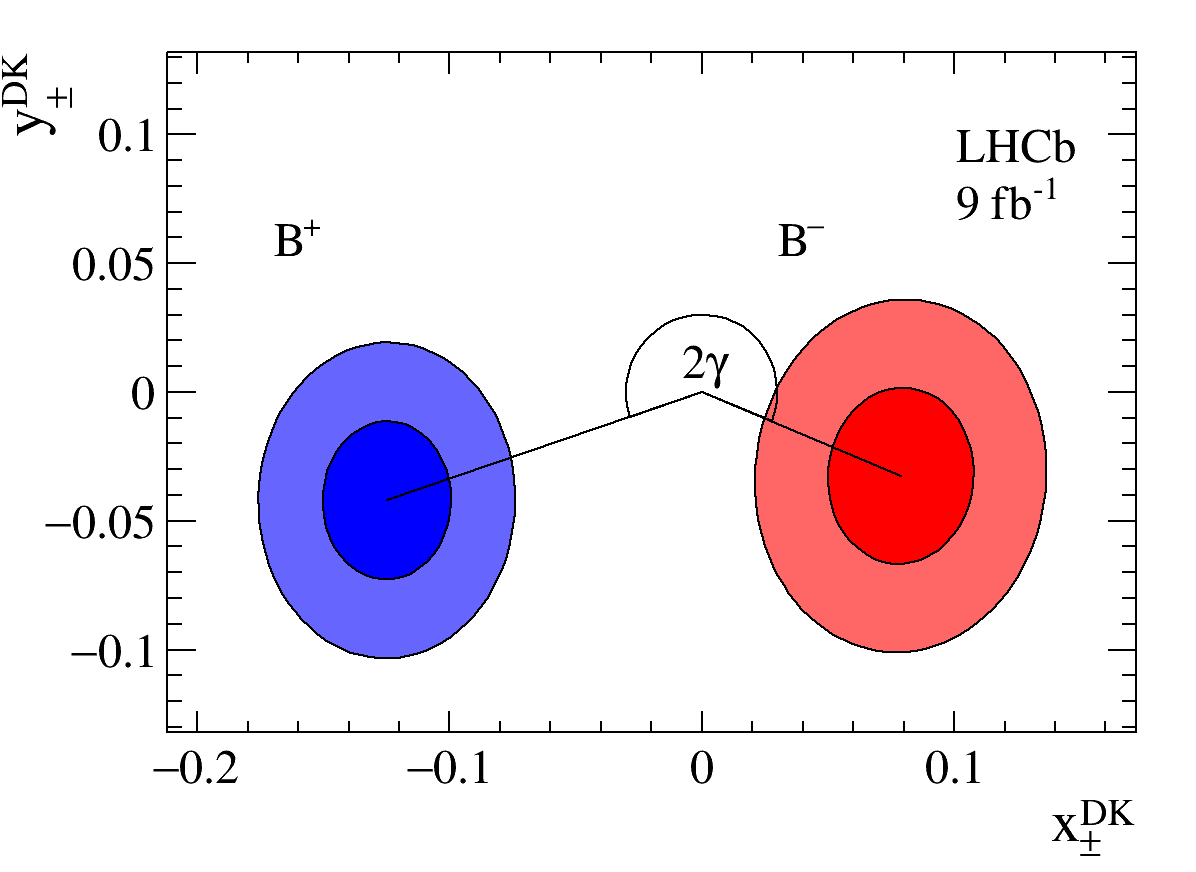
\includegraphics[width = 1.0\textwidth]{Plots/B2DK_CP_Observables_Contours.png}
      \caption{$x_\pm^{DK}$ vs $y_\pm^{DK}$}
    \end{subfigure}%
    \begin{subfigure}{0.5\textwidth}
      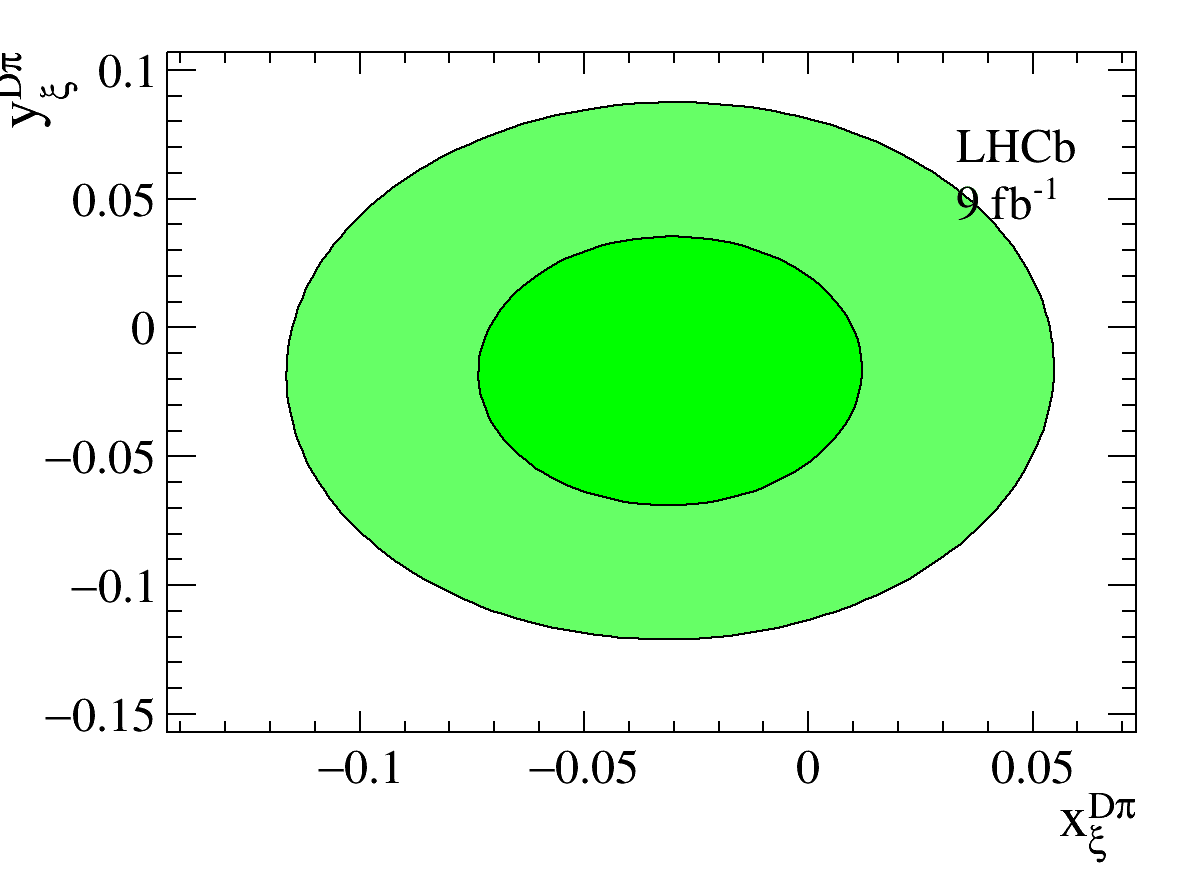
\includegraphics[width = 1.0\textwidth]{Plots/B2Dpi_CP_Observables_Contours.png}
      \caption{$x_\xi^{D\pi}$ vs $y_\xi^{D\pi}$}
    \end{subfigure}
  \end{figure}
\end{frame}

\begin{frame}{Fractional bin asymmetries}
  \begin{figure}
    \centering
    \vspace{-0.2cm}
    \begin{subfigure}{0.5\textwidth}
      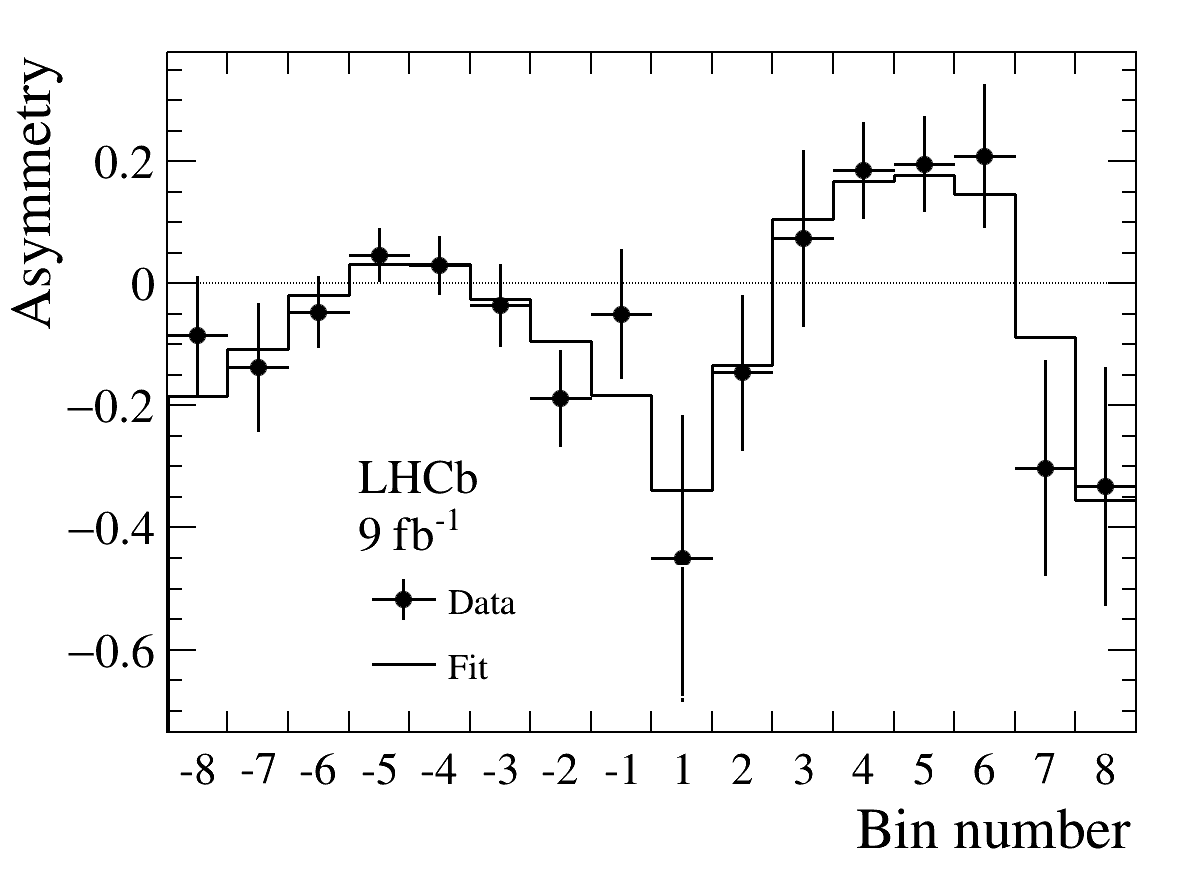
\includegraphics[width = 1.0\textwidth]{Plots/BinAsymmetries_dk.png}
      \caption{$B^\pm\to DK^\pm$}
    \end{subfigure}%
    \begin{subfigure}{0.5\textwidth}
      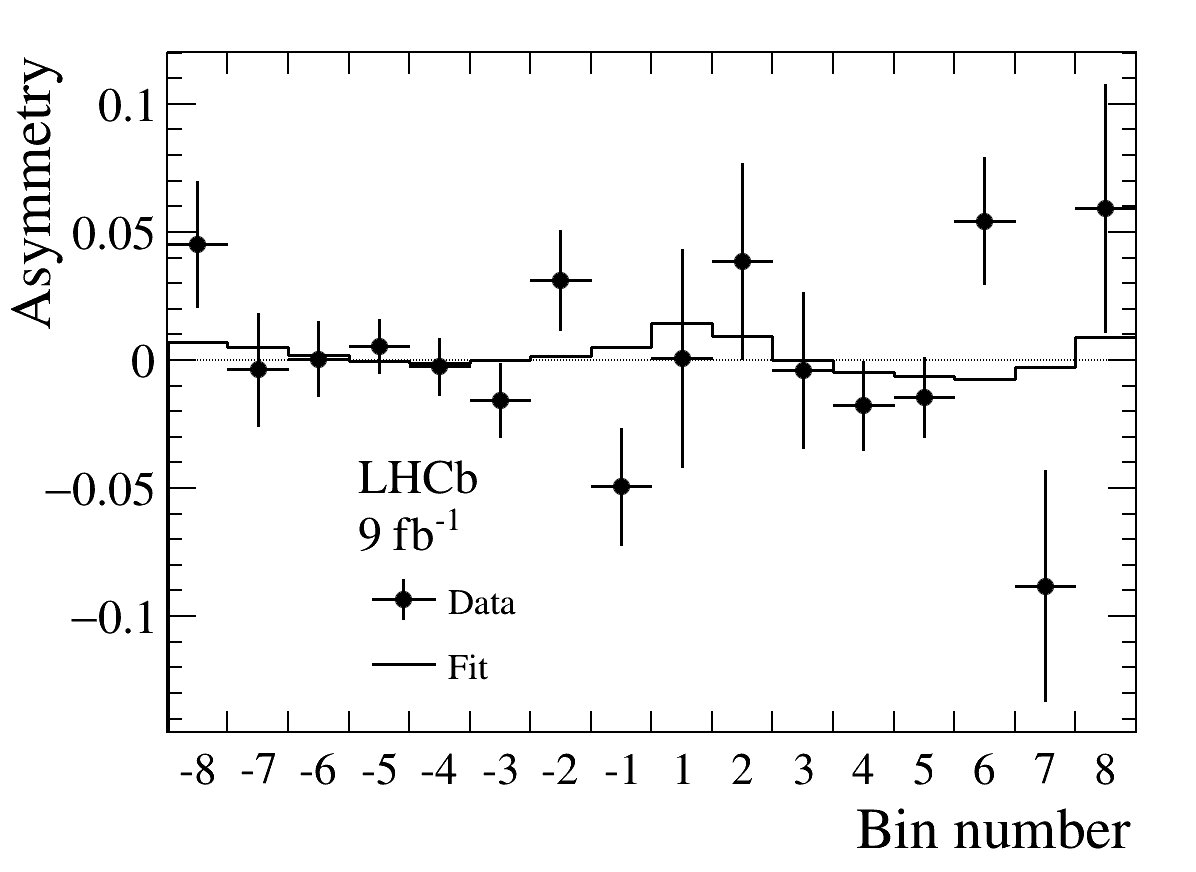
\includegraphics[width = 1.0\textwidth]{Plots/BinAsymmetries_dpi.png}
      \caption{$B^\pm\to D\pi^\pm$}
    \end{subfigure}
  \end{figure}
\end{frame}

\subsection{Systematic uncertainties}
\begin{frame}{Systematic uncertainties}
  \begin{itemize}
    \setlength\itemsep{1.0em}
    \item{Dominant $c_i$/$s_i$ systematic uncertainty due to model dependence}
    \begin{itemize}
      \item{Strategy: Generate toys with $c_i$/$s_i$ from older CLEO model, fit with $c_i$/$s_i$ from LHCb model}
      \item{Will be replaced when BESIII results become available}
    \end{itemize}
    \item{All internal systematic uncertainties are much smaller than the statistical uncertainties}
  \end{itemize}
\end{frame}

\begin{frame}{Summary of all BPGGSZ systematic uncertainties}
  \begin{center}
    Uncertainties of BPGGSZ CP observables in units of $10^{-2}$
  \end{center}
  \scriptsize
  \vspace{0.02cm}
  \begin{center}
    \begin{tabular}{lcccccc} 
      \hline
      Source & $x_-^{DK}$ & $y_-^{DK}$ & $x_+^{DK}$ & $y_+^{DK}$ & $x_\xi^{D\pi}$ & $y_\xi^{D\pi}$ \\
      \hline
      Statistical                                   & 2.99  & 3.50  & 2.58  & 3.10  & 4.07  & 4.89  \\
      \hline
      $c_i$, $s_i$                                  & 0.14  & 3.82  & 1.78  & 1.03  & 0.01  & 0.71  \\
      \hline
      $B^\pm\to D\mu\nu$   background               & 0.07  & 0.06  & 0.08  & 0.30  & 0.17  & 0.00  \\
      $D\to K(X)l\nu_l$ background                  & 0.08  & 0.00  & 0.73  & 0.14  & 0.27  & 0.44  \\
      $D\to K\pi\pi\pi$ background                  & 0.25  & 0.00  & 0.73  & 0.06  & 0.07  & 0.27  \\
      $D\to K\pi\pi\pi\pi^0$ background             & 0.37  & 0.07  & 0.20  & 0.04  & 0.45  & 0.19  \\
      $\Lambda_b$ background                        & 0.10  & 0.06  & 0.06  & 0.26  & 0.15  & 0.07  \\
      Bin dependent mass shape                      & 0.06  & 0.12  & 0.13  & 0.12  & 0.24  & 0.12  \\
      Charmless background                          & 0.15  & 0.18  & 0.14  & 0.16  & 0.01  & 0.01  \\
      Fit bias                                      & 0.00  & 0.00  & 0.00  & 0.00  & 0.00  & 0.00  \\
      Fixed yield fractions                         & 0.02  & 0.03  & 0.02  & 0.02  & 0.01  & 0.01  \\
      Low mass physics effects                      & 0.15  & 0.21  & 0.05  & 0.20  & 0.03  & 0.44  \\
      Mass shape                                    & 0.03  & 0.03  & 0.02  & 0.02  & 0.04  & 0.01  \\
      PID Efficiency                                & 0.03  & 0.03  & 0.02  & 0.02  & 0.04  & 0.01  \\
      $D$ mixing                                    & 0.00  & 0.02  & 0.01  & 0.02  & 0.00  & 0.00  \\
      \hline
      Total LHCb systematic                         & 0.52  & 0.32  & 1.08  & 0.52  & 0.63  & 0.72  \\
      \hline
      Total systematic                              & 0.54  & 3.83  & 2.08  & 1.15  & 0.63  & 1.01  \\
      \hline
    \end{tabular}
  \end{center}
\end{frame}

\begin{frame}{Summary of all quasi-GLW systematic uncertainties}
  \begin{center}
    Uncertainties of quasi-GLW CP observables in units of $10^{-2}$
  \end{center}
  \footnotesize
  \vspace{0.02cm}
  \begin{center}
    \begin{tabular}{lcccccc} 
      \hline
      Source & $A_K^{KK\pi\pi}$ & $A_\pi^{KK\pi\pi}$ & $A_K^{\pi\pi\pi\pi}$ & $A_\pi^{\pi\pi\pi\pi}$ & $R_{\rm CP}^{KK\pi\pi}$ & $R_{\rm CP}^{\pi\pi\pi\pi}$ \\
      \hline
      Statistical                                   & 23.49 & 13.36 &  5.56 &  3.12 & 24.54 & 14.46 \\
      \hline
      Charmless background                          &  1.20 &  0.44 &  0.01 &  0.00 & 13.72 &  8.43 \\
      External parameters                           &  0.98 &  0.99 &  0.74 &  0.74 &  3.98 &  3.96 \\
      Fixed yield fractions                         &  0.11 &  0.08 &  0.02 &  0.00 &  1.32 &  1.44 \\
      Mass shape                                    &  0.27 &  0.20 &  0.03 &  0.02 &  3.11 &  3.05 \\
      PID efficiency                                &  0.18 &  0.12 &  0.01 &  0.00 &  2.55 &  1.64 \\
      \hline
      Total systematic                              &  1.59 &  1.11 &  0.74 &  0.74 & 14.90 & 10.04 \\
      \hline
    \end{tabular}
  \end{center}
\end{frame}

\section{Interpretation}

\begin{frame}{Interpretation}
  \begin{figure}
    \centering
    \begin{subfigure}{0.50\textwidth}
      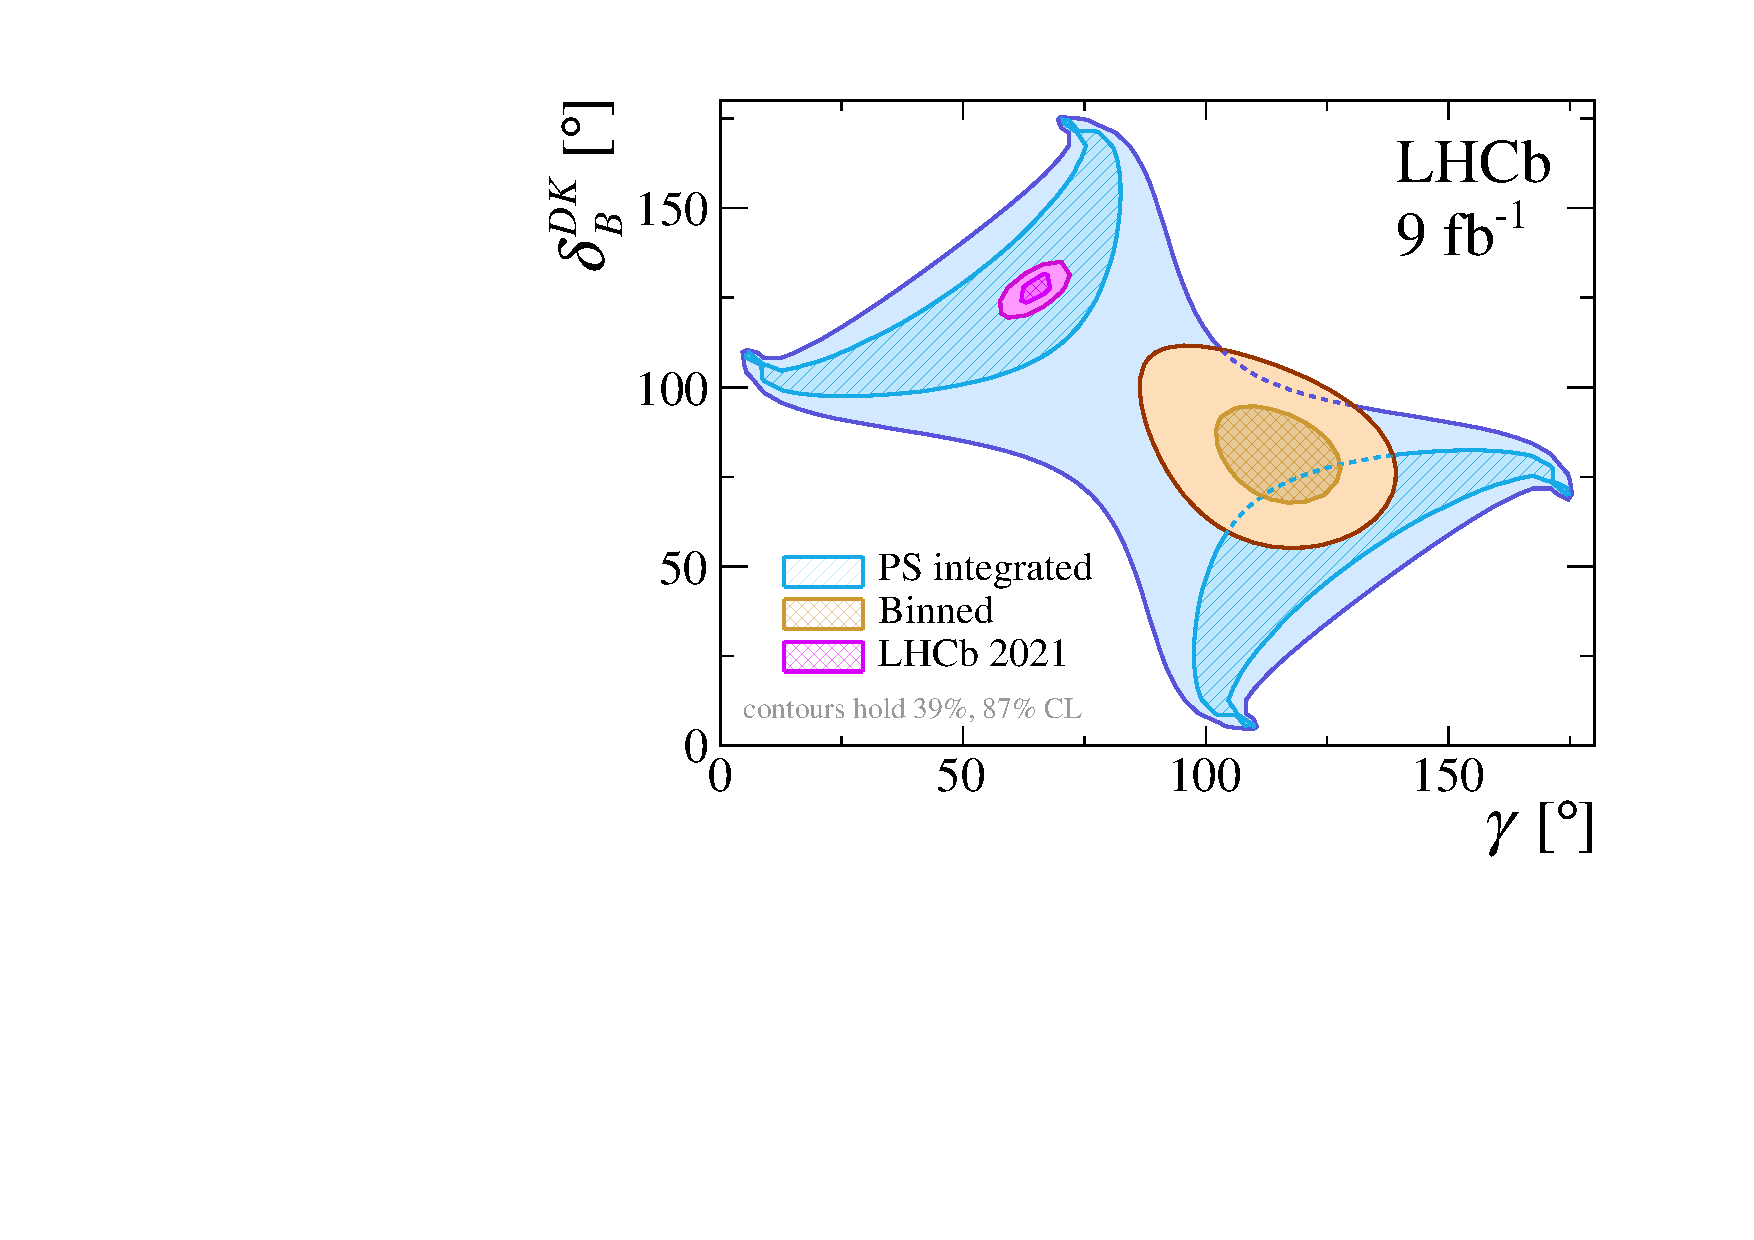
\includegraphics[width = 1.0\textwidth]{Plots/gammacharm_lhcb_KKpipi_GLW_KKpipi_GGSZ_lhcb_2020_beauty_and_charm_g_d_dk.pdf}
    \end{subfigure}%
    \begin{subfigure}{0.50\textwidth}
      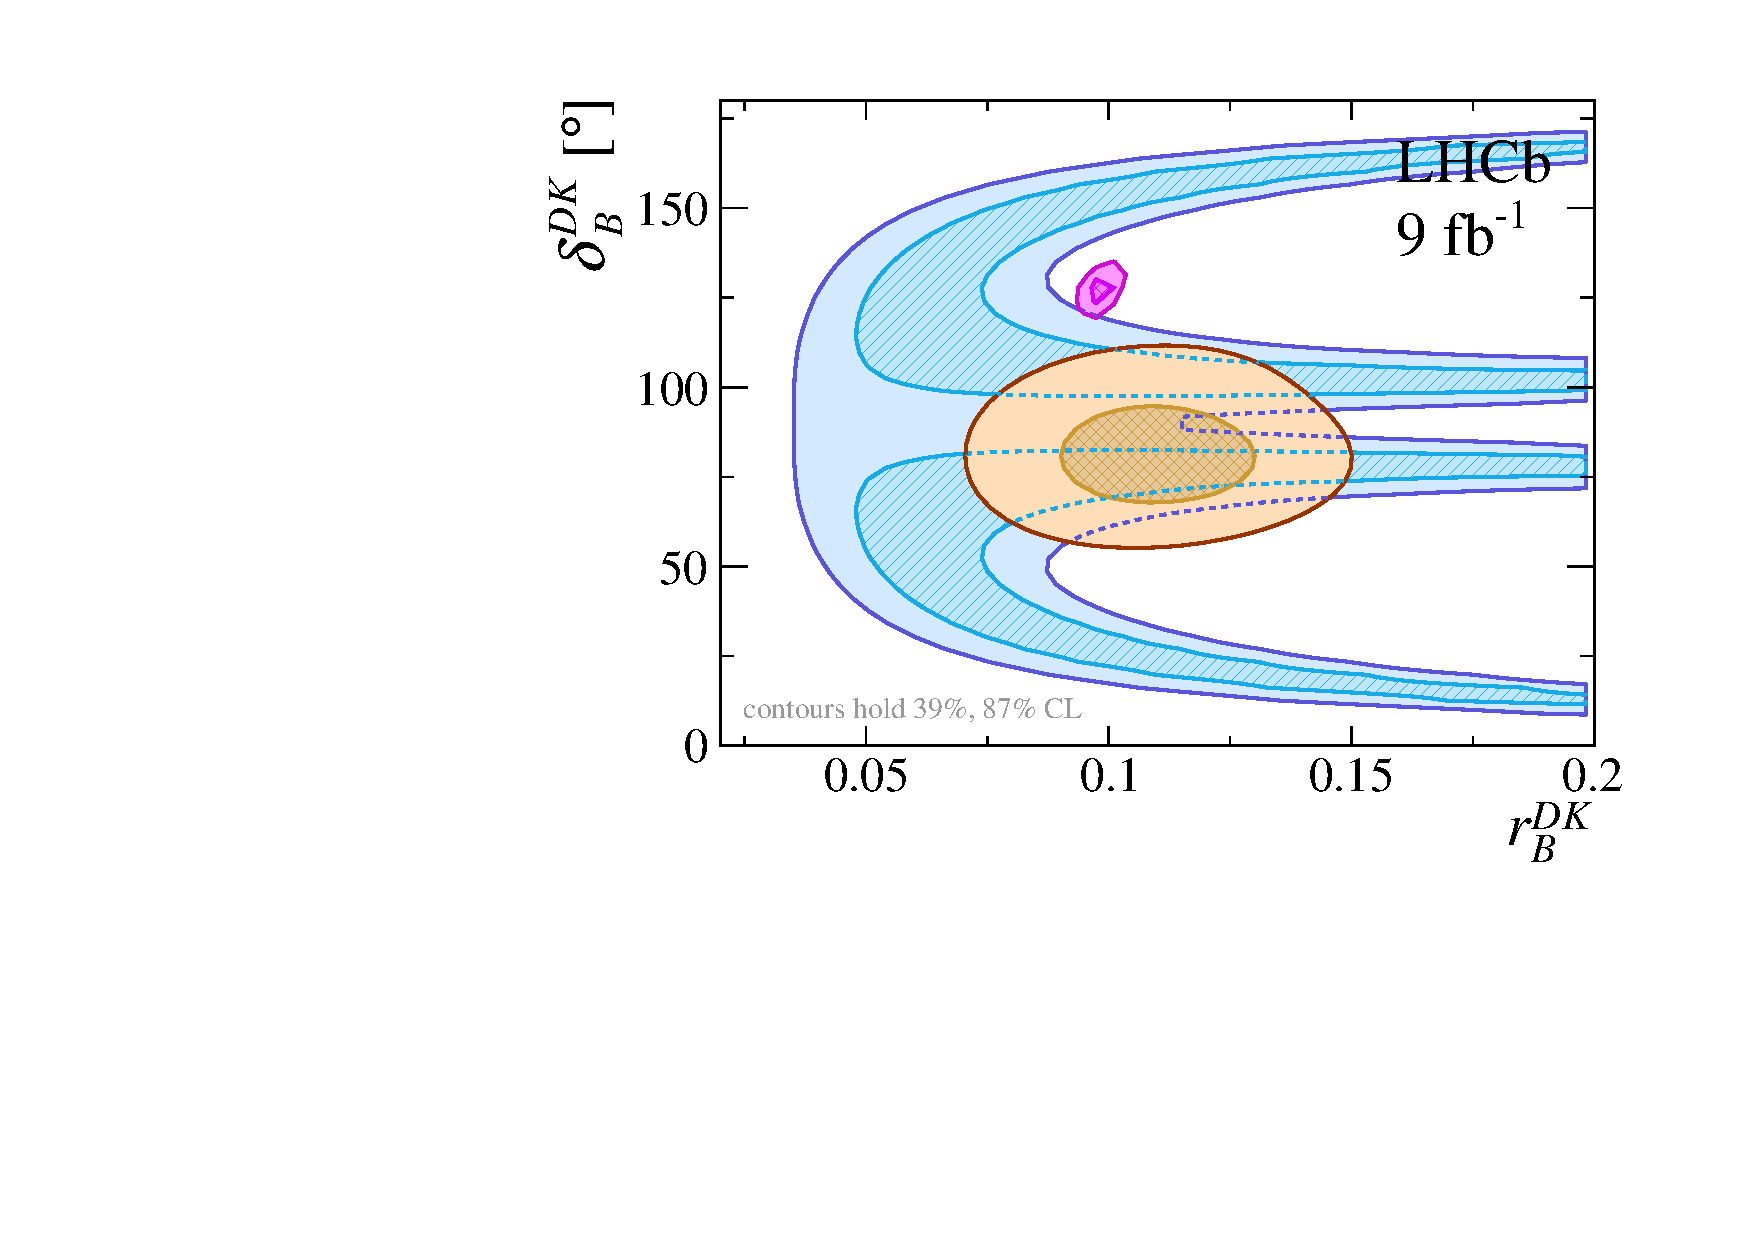
\includegraphics[width = 1.0\textwidth]{Plots/gammacharm_lhcb_KKpipi_GLW_KKpipi_GGSZ_lhcb_2020_beauty_and_charm_r_dk_d_dk.pdf}
    \end{subfigure}
  \end{figure}
  \vspace{-0.75cm}
  \begin{align*}
    \gamma =& (103\pm14)^\circ \\
    \delta_B^{DK} =& (92\pm14)^\circ \\
    r_B^{DK} =& 0.117\pm0.020 \\
    \delta_B^{D\pi} =& (296\pm84)^\circ \\
    r_B^{D\pi} =& 0.004\pm0.005
  \end{align*}
\end{frame}

\section{Summary}

\begin{frame}{Summary}
  \begin{itemize}
    \item{Measured CP observables:}
  \end{itemize}
  \vspace{-0.2cm}
  \begin{align*}
    x_-^{DK} =& (8.3 \pm 3.0 \pm 0.5 \pm 0.1)\times 10^{-2}, \\
    y_-^{DK} =& (-1.2 \pm 3.5 \pm 0.3 \pm 3.8)\times 10^{-2}, \\
    x_+^{DK} =& (-13.5 \pm 2.6 \pm 1.1 \pm 1.8)\times 10^{-2}, \\
    y_+^{DK} =& (-4.0 \pm 3.1 \pm 0.5 \pm 1.0)\times 10^{-2}, \\
    x_\xi^{D\pi} =& (-2.9 \pm 4.1 \pm 0.6 \pm 0.0)\times 10^{-2}, \\
    y_\xi^{D\pi} =& (-2.0 \pm 4.9 \pm 0.7 \pm 0.7)\times 10^{-2},
  \end{align*}
  \vspace{-0.5cm}
  \begin{itemize}
    \item{Measured physics parameters:}
  \end{itemize}
  \vspace{-0.2cm}
  \begin{align*}
    \gamma =& (103\pm14)^\circ \\
    \delta_B^{DK} =& (92\pm14)^\circ \\
    r_B^{DK} =& 0.117\pm0.020 \\
    \delta_B^{D\pi} =& (296\pm84)^\circ \\
    r_B^{D\pi} =& 0.004\pm0.005
  \end{align*}
\end{frame}

\section{Conclusion}

\begin{frame}{Conclusion}
  \begin{itemize}
    \setlength\itemsep{2em}
    \item{First study of CP violation has been performed in $B^\pm\to[K^+K^-\pi^+\pi^-]_D h^\pm$ in bins of phase space}
    \item{Phase space inclusive measurement for $B^\pm\to[K^+K^-\pi^+\pi^-]_D h^\pm$ and $B^\pm\to[\pi^+\pi^-\pi^+\pi^-]_D h^\pm$}
    \item{This publication is model dependent, but strong phases will be available from BESIII soon}
  \end{itemize}
  \begin{center}
    \Huge Thank you!
  \end{center}
\end{frame}

\end{document}